\documentclass{pginz}

%%%%%%%%%Miejsce na dodatkowe pakiety%%%%%%%%%%%%%
\usepackage{subcaption}
\usepackage{pdfpages}
\usepackage[T1]{fontenc}
\usepackage{csquotes}
\usepackage{float}
\usepackage{hyperref}
\usepackage[
    backend=biber,
    style=numeric,
    sorting=none,
    sortcites=true,
    maxnames=99,
    minnames=1,
    backref=false,
    natbib=true
]{biblatex}
\addbibresource{literatura.bib}

\addto\captionspolish{
  \renewcommand{\listfigurename}{Wykaz rysunków}
  \renewcommand{\listtablename}{Wykaz tabel}
}

\begin{document}

% \includepdf[pages={1}]{StronaTytulowa.pdf}

% \includepdf[page={1-2}]{Oswiadczenie.pdf}

\setcounter{page}{4}

\chapter*{Streszczenie}
Prezentowana praca dyplomowa skupia się na przedstawieniu różnic w użytkowaniu dużych modeli językowych, będących częścią wybranych konfiguracji systemów RAG. Autor zaprezentował przebieg i wyniki badania, które miało na celu sprawdzić wydajność tych algorytmów podczas przetwarzania pytań, dotyczących zewnętrznych nieustrukturyzowanych i ustrukturyzowanych źródeł danych. W tym celu, utworzono oprogramowanie do testów i interfejs, umożliwiający prowadzenie konwersacji z dwoma wybranymi optymalnymi systemami.

Część teoretyczna składa się z wprowadzenia do przetwarzania języka naturalnego, dużych modeli językowych oraz techniki generowania wspomaganego wyszukiwaniem. Scharakteryzowano między innymi: zarys historyczny chatbotów, sposób w jaki maszyny rozumieją ludzki język oraz jak działają LLMy i dlaczego są one chętnie wykorzystywane w ramach RAG.

Część związana z przeglądem literatury opisuje w jaki sposób naukowcy podchodzą do ewaluacji systemów RAG. Pierwsza przywołana publikacja zaprezentowała skalowalny wielodokumentowy test wydajnościowy MEBench. W drugim artykule autorzy pochylili się nad benchmarkiem RGB, w ramach którego przetestowano systemy RAG tysiącem pytań z czterech kategorii: odporność na szum, odmowa odpowiedzi, integracja informacji i odporność na błędne fakty. Natomiast, w trzeciej publikacji opisano benchmark NL-to-SQL, składający się łącznie z 360 łatwych, umiarkowanych i trudnych pytań odnoszących się do bazy danych SQL.

W części badawczej przedstawiono autorskie oprogramowanie umożliwiające automatyzację testowania trzydziestu różnych systemów RAG. Autor dokładnie opisał jak powstały dane nieustrukturyzowane w postaci pliku PDF i tekstowego  oraz dane ustrukturyzowane w postaci bazy danych SQL i pliku CSV. Inspirując się przestudiowaną literaturą, zaproponowano dwa zestawy ośmiu pytań, dedykowanych dwóm typom wyżej wymienionych źródeł informacji.

Część, w której skupiono się na analizie wyników badania, prezentuje porównanie systemów RAG pod kątem trafności generowanych odpowiedzi, kosztu ich uzyskania, czasu generowania oraz przepustowości tokenów. W ostatnim kroku, wybrano dwa najwydajniejsze systemy, po jednym z każdej kategorii. Następnie zintegrowano je z graficznym interfejsem użytkownika, co umożliwiło prowadzenie z nimi konwersacji.



\bigskip
\bigskip

\noindent \textbf{Słowa kluczowe}: \\
NLP, Chatbot, sztuczna inteligencja, LLM, RAG, agent AI, dane nieustrukturyzowane, dane ustrukturyzowane, PDF, plik tekstowy, SQL, CSV, automatyzacja, GUI, scraping, embedder, wektorowa baza danych


\bigskip

\noindent \textbf{Dziedzina nauki i techniki, zgodnie z wymogami OECD}: \\
Nauki inżynieryjne i techniczne, informatyka techniczna i telekomunikacja
\chapter*{Abstract}

The Master's Thesis focuses on presenting the differences in usage of large language models, which belong to different configurations of RAG systems. The author has presented process and results of the research in terms of the algorithms' performance while answering questions related to external unstructured and structured data sources. To this end, the author has created a test workflow and an interface enabling conversation with the two chosen optimal systems.

The theory section introduces a reader to natural language processing, large language models and retrieval-augmented generation technique. There were described: history of chatbots, the way machines understand human language, how LLMs work and why they are eagerly used in RAG systems.

The chapter dedicated to literature review shows the scientists' approach to RAG systems evaluation. First reffered publication presented a scalable multi-document performance test called MEBench. In the second one, the authors delved into the topic of RGB benchmark, which enabled testing RAG systems with 1000 questions from four categories: noise robustness, negative rejection, information integration and counterfactual robustness. However, the third article focused on NL-to-SQL benchmark, which consisted of altogether 360 simple, moderate and challenging questions related to SQL database.

In the research part, the author has presented his original workflow enabling test automation of thirty different RAG systems. The creation process of unstructured data (PDF and text file) and structured data (SQL database and CSV file) was also described. Inspired by studied literature, the author proposed two sets of eight questions dedicated to two of the mentioned types of information sources.

The last section focuses on results analysis and presents comparison of RAG systems in terms of accuracy and cost of generated answers, time of generation and token throughput. In the last step, the two most efficient systems were chosen, one from each category. Then, the author has integrated them with a graphical user interface, enabling interaction through conversation.



\bigskip
\bigskip

\noindent \textbf{Key words}: \\
NLP, Chatbot, artificial intelligence, LLM, RAG, AI agent, unstructured data, structured data, PDF, text file, SQL, CSV, automation, GUI, scraping, embedder, vector database


\bigskip

\noindent \textbf{Field of science and technology as required by the OECD}: \\
Engineering and Technical Sciences, Technical Computer Science and Telecommunications

\tableofcontents
\addcontentsline{toc}{chapter}{Wykaz ważniejszych oznaczeń i skrótów}

%\include{Symbole}
\chapter*{Wykaz ważniejszych oznaczeń i skrótów}


\begin{itemize}
[noitemsep,topsep=0pt,parsep=0pt,partopsep=0pt,labelwidth=1cm,align=left,itemindent=0pt]

    \item[NLP] - Natural Language Processing
    \item[NL] - Natural Language
    \item[ML] - Machine Learning
    \item[XML] - Extensible Mark-up Language
    \item[AIML] - Artificial Intelligence Markup Language
    \item[AI] - Artificial Intelligence
    \item[GenAI] - Generatywna Sztuczna Inteligencja 
    \item[UE] - Unia Europejska
    \item[GRU] - Gated Recurrent Unit
    \item[LLM] - Large Language Model
    \item[RAG] - Retrieval-Augmented Generation
    \item[API] - Application Programming Interface
    \item[MEBench] - Multi-Entity Benchmark
    \item[SQL] - Structured Query Language
    \item[SLM] - Small Language Model
    \item[ACM] - Association for Computing Machinery
    \item[FT] - Fine-Tuned
    \item[QA] - Quality Assurance
    \item[RGB] - Retrieval-Augmented Generation Benchmark 
    \item[ZIP] - Format bezstratnej kompresji danych
    \item[URL] - Uniform Resource Locator
    \item[HTTP] - Hypertext Transfer Protocol
    
\end{itemize}


\cleardoublepage

\chapter{Wstęp i cel pracy}
Od 2022 roku duże modele językowe stały się nieodłącznym narzędziem w życiu każdego człowieka, ułatwiając codzienne zadania. Każdego roku ukazują się nowe, bardziej zaawansowane i przełomowe LLMy. Obecnym trendem w świecie biznesu jest zastosowanie komercyjnych modeli, zapewniając im dostęp do wewnętrznej dokumentacji, baz danych czy repozytoriów kodu. W takiej sytuacji użytkownik lub firma stoi przed wyborem optymalnego rozwiązania, które jest możliwie skuteczne, tanie i szybko działające. Stąd, w tym dynamicznym środowisku, wychodzi potrzeba cyklicznego testowania i porównywania najnowszych popularnych algorytmów biorąc pod uwagę powyższe kryteria.


    \section{Cel pracy}
    Celem pracy magisterskiej jest stworzenie projektu, analiza wydajności oraz implementacja rozwiązania, umożliwiającego ekstrakcję i agregację danych z ustrukturyzowanych i nieustrukturyzowanych źródeł informacji. W ramach powyższych aktywności należy wykorzystać podejście Retrieval-Augmented Generation (RAG) współpracujące z dużymi modelami językowymi. W ramach ewaluacji skuteczności rozwiązania wskazane jest  przeprowadzenie testów porównawczych różnych wariantów systemów RAG, które obejmują m.in.: techniki podziału dokumentów (chunking), różne embeddery, zastosowanie wektorowych baz danych oraz wybranych popularnych najnowszych modeli językowych. W zakresie analizy skuteczności wskazane jest przeprowadzenie oceny w obszarze trafności odpowiedzi, kosztu generacji (tokenów), czasu odpowiedzi, odporności na pytania spoza kontekstu oraz zdolności algorytmów do odmowy udzielenia odpowiedzi w przypadku braku wystarczającej ilości danych. Najlepiej dobrana konfiguracja RAG powinna zostać udostępniona poprzez graficzny interfejs użytkownika, umożliwiając użytkownikowi zadawanie pytań opartych na dostępie do własnych źródeł danych. Opracowane rozwiązanie powinno wspierać generowanie spersonalizowanych rekomendacji dla odbiorców zainteresowanych konkretnymi aspektami usług lub informacji w wybranym obszarze tematycznym.
\cleardoublepage

\chapter{Wprowadzenie do przetwarzania języka naturalnego}
W tym rozdziale przedstawiono podstawowe definicje i pojęcia kryjące się za terminem \enquote{przetwarzanie języka naturalnego} (ang. \textit{natural language processing — NLP}). Zaprezentowano także ewolucję chatbotów i różne podejścia do rozwoju NLP ze szczególnym uwzględnieniem metod uczenia maszynowego.


    \section{Definicja przetwarzania języka naturalnego}
    Określenie \enquote{język naturalny} stosuje się, aby odseparować język ludzki (np. polski, włoski czy chiński) od języka formalnego (np. Python, C++ czy XML). Język naturalny był rozwijany przez ludzi na drodze długofalowej ewolucji. Służy do komunikacji oraz wyrażania myśli i emocji w formie werbalnej. Język formalny zaś, składający się z symboli przystępnych do zrozumienia dla człowieka, zapewnia doskonałą komunikację między programistą a maszyną. Dzięki swojej precyzji umożliwia tworzenie m.in. zaawansowanych aplikacji komputerowych oraz skryptów.
    
    Przetwarzanie języka naturalnego  to technika pozwalająca komputerom interpretować i generować ludzki język. NLP umożliwia maszynom analizę ludzkich słów i reagowanie na nie w sposób sensowny i naturalny. Tą interdyscyplinarną technikę tworzą trzy główne dziedziny: sztuczna inteligencja, informatyka oraz lingwistyka. Przedstawiono to na diagramie \ref{nlp_diagram}.

    \begin{center}
        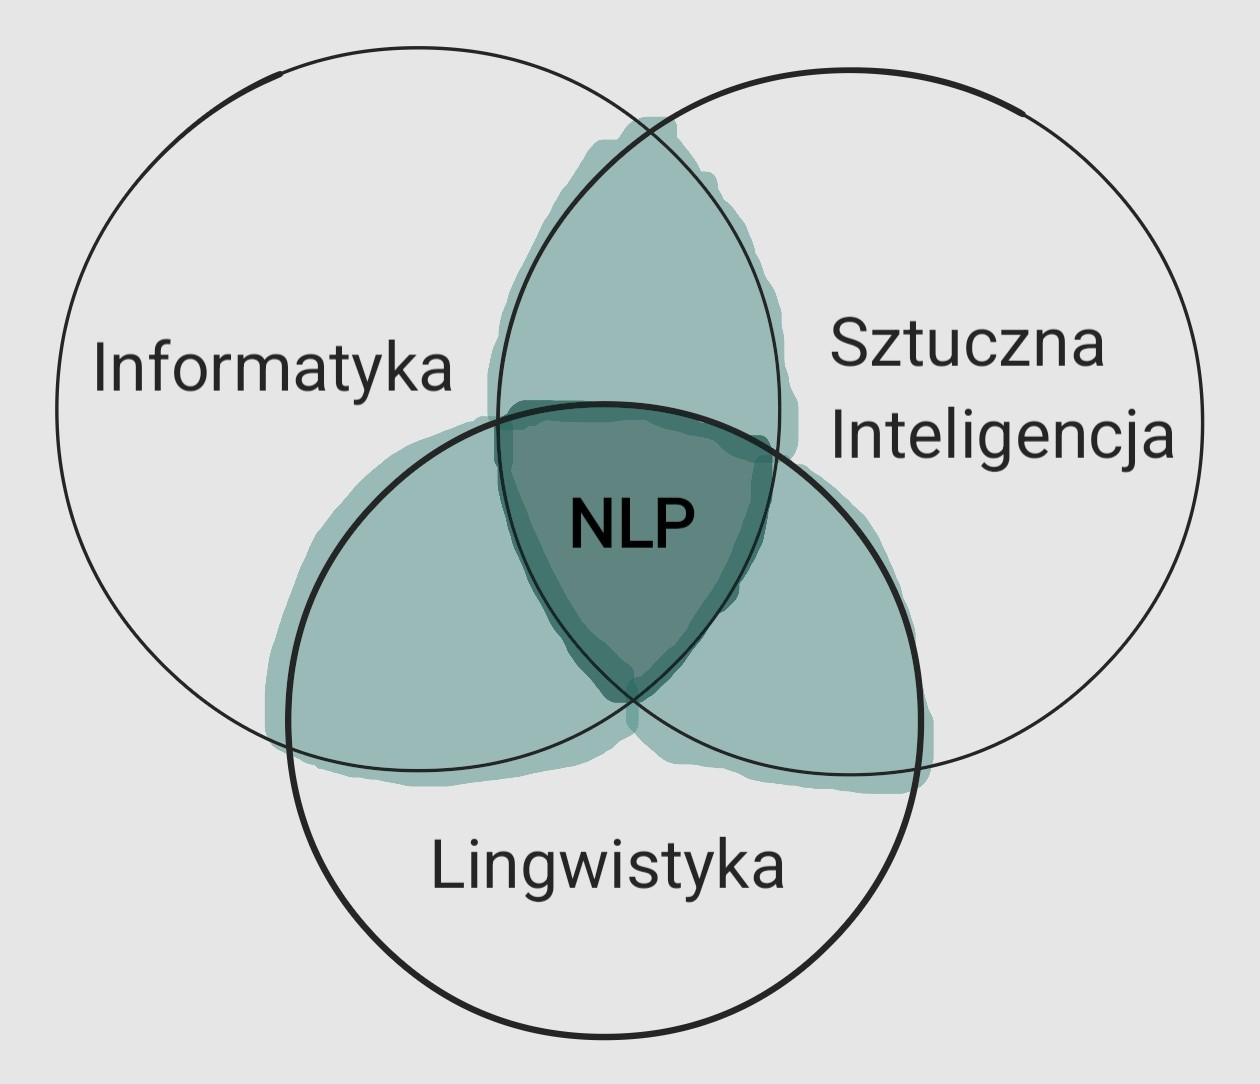
\includegraphics[width=0.5\textwidth]{rysunki/nlp_diagram.jpg}
        \captionof{figure}{ Diagram przedstawiający trzy dziedziny, które współtworzą przetwarzanie języka naturalnego \cite{krohn2022uczenie} }
        \label{nlp_diagram}
    \end{center}

    Przetwarzanie języka naturalnego stosuje się zarówno w kontekście języka pisanego, jak i mówionego. Technologie i algorytmy z tej dziedziny mają swoje zastosowania w następujących obszarach:
    \begin{itemize}
        \item tłumaczenie z jednego języka na inny,
        \item analiza sentymentu,
        \item wyszukiwarki kontekstowe,
        \item prowadzenie konwersacji z komputerem (chatboty).
    \end{itemize}


    \section{Definicja chatbota}
    Chatbotem nazywa się oprogramowanie wykorzystujące NLP, które za pomocą interfejsu graficznego lub głosowego umożliwia człowiekowi konwersację z komputerem, do złudzenia przypominającą rozmowę dwóch użytkowników. Chociaż początki tego rozwiązania sięgają już połowy dwudziestego wieku, to dopiero w ostatnich latach stały się one bardzo popularne i przełomowe w obszarze sztucznej inteligencji za sprawą wykorzystania dużych modeli językowych.
    
    
    \section{Zarys historyczny chatbotów}
    Znaczący wkład w rozwój przetwarzania języka naturalnego, w tym chatbotów, wniósł w 1950 roku brytyjski matematyk i informatyk Alan Turing. W artykule \enquote{Computing Machinery and Intelligence} pionier szukał odpowiedzi na pytanie \enquote{Czy maszyny potrafią myśleć?} \cite{turing1950}. W ramach tego zagadnienia, stworzył test, który nazwano testem Turinga. Polegał on na tym, że osoba badana, inaczej zwana sędzią, prowadziła dwie konwersacje: jedną z drugim człowiekiem, a drugą z komputerem. Jeżeli badany nie był w stanie jednoznacznie rozróżnić, który dialog był prowadzony z chatbotem, komputer pozytywnie przechodził test.

    
        \subsection{ELIZA}
        W 1966 roku niemiecki informatyk Joseph Weizenbaum, zainspirowany testem Turinga, napisał w języku SLIP program symulujący konwersację z psychoanalitykiem. Chatbot został nazwany ELIZA na cześć głównej bohaterki dramatu Pigmalion, Elizy Doolittle. Program używał prostych technik rozpoznawanie słów kluczowych, dopasowania wzorców (ang. \textit{pattern matching}) i mechanizmu substytucji. Poniżej przedstawiono przykładowy dialog, prezentujący jak ELIZA przekształcała zdania użytkownika w swoich odpowiedziach \cite{from_eliza_to_chatgpt2024}:

        \begin{enumerate}
            \item You: Well, my boyfriend made me come here.\newline
                ELIZA: Is it important to you that your boyfriend made you come here ?
            \item You: He says I'm depressed much of the time.\newline
                ELIZA: I am sorry to hear that you are depressed.
            \item You: It is true. I'm unhappy.\newline
                ELIZA: Can you explain what made you unhappy ?
        \end{enumerate}

        Trudności w odróżnieniu chatbota od drugiego człowieka spowodowały, że niektórzy użytkownicy za bardzo przywiązywali się do programu, wierząc, że ich rozumie. Rezultatem tego, było zdefiniowanie zjawiska psychologicznego, które nazwano efektem Elizy. Polega ono na tym, że człowiek przypisuje maszynie ludzkie cechy, takie jak empatię, zrozumienie czy inteligencję.


        \subsection{PARRY}
        W 1972 roku amerykański psychiatra Kenneth Colby napisał w języku MLISP program PARRY. Konwersacja z tym chatbotem miała imitować prowadzenie dialogu z osobą chorą na schizofrenię paranoidalną. Jego zadaniem były prowokacja i wprowadzanie kontrowersji, które miały skłonić użytkownika do pisania dłuższych wypowiedzi \cite{history_of_chatbots2019}. Odpowiedzi programu bazowały na zbiorze zasad zdefiniowanych w logice systemu i były one generowane za pomocą techniki “elaboration” \cite{from_eliza_to_chatgpt2024}. PARRY był znacznie bardziej zaawansowanym rozwiązaniem niż ELIZA.


        \subsection{A.L.I.C.E.}
        Program Artificial Linguistic Internet Computer Entity (ALICE) został napisany w 1995 w języku Java przez amerykańskiego informatyka Richarda Wallace'a. Baza wiedzy systemu przechowywana była w plikach AIML, stanowiących implementację standardu XML. W latach 1995-2000 społeczność Alicebot zapewniła funkcjonalność, umożliwiającą użytkownikom dodawanie wzorców konwersacyjnych do bazy wiedzy chatbota \cite{alice2015}. Inteligencja ALICE opierała się na zaawansowanym dopasowywaniu wzorców.


        \subsection{SmarterChild}
        W 2001 roku firma ActiveBuddy udostępniła do powszechnego użytku chatbota SmarterChild. Użytkownicy mogli prowadzić dialog z cyfrowym asystentem za pomocą platform: AOL Instant Messenger, Windows Live Messenger oraz Yahoo Messenger. Nie tylko odpowiadał on na pytania dotyczące pogody, sportu czy najnowszych wiadomości, ale także grał w gry. System był w stanie uczyć się i ewoluować wraz z każdą interakcją z człowiekiem. Pozwalało mu to na dostosowywanie stylu odpowiedzi znając styl pisania i preferencje użytkownika \cite{from_eliza_to_chatgpt2024}.
    

        \subsection{Siri}
        W 2011 roku firma Apple zaprezentowała Siri, przełomowego asystenta AI, który do dziś jest powszechnie używany w produktach koncernu. Komponując ze sobą przetwarzanie języka naturalnego i uczenie maszynowe, Siri jest w stanie przeanalizować zapytanie użytkownika i zapewnić odpowiednią, spersonalizowaną odpowiedź. Wirtualny asystent pomaga w wykonywaniu najróżniejszych zadań w smartfonie, takich jak wysłanie wiadomości, zestawienie połączeń czy ustawienie budzika \cite{from_eliza_to_chatgpt2024}.

        
    \section{Podejścia do przetwarzania języka naturalnego}
    Metody rozwiązywania problemów NLP można podzielić na trzy rodzaje: heurystykę, uczenie maszynowe oraz uczenie głębokie. W tym podrozdziale zwięźle przedstawiono każde z tych podejść.

        \subsection{Metody heurystyczne}
        We wczesnych systemach przetwarzania języka naturalnego oprócz słowników i tezaurusów rozwijano także bardziej złożone bazy wiedzy wspomagające NLP oparte na regułach. Doskonale obrazuje to WordNet \cite{wordnet_d3}. Jest to baza słów i semantycznych relacji między nimi. Do takich relacji zalicza się:

        \begin{itemize}
            \item synonimy — wyrażenia o takim samym lub zbliżonym znaczeniu, które brzmią i zapisuje się inaczej,
            \item hiponimy — słowa o znaczeniu węższym, które nazywają konkretny rodzaj lub gatunek obiektu z szerszej grupy, np. \enquote{arabski} i \enquote{chiński} to hiponimy języka obcego,
            \item meronimy — słowa nazywające część składową, która współtworzy większą całość, np. \enquote{silnik} i \enquote{kierownica} to meronimy samochodu.
        \end{itemize}

        \noindent Na rysunku \ref{heurystyka_transport_publiczny} przedstawiono wizualizację takich relacji między słowami w bazie WordNet.

        \begin{center}
            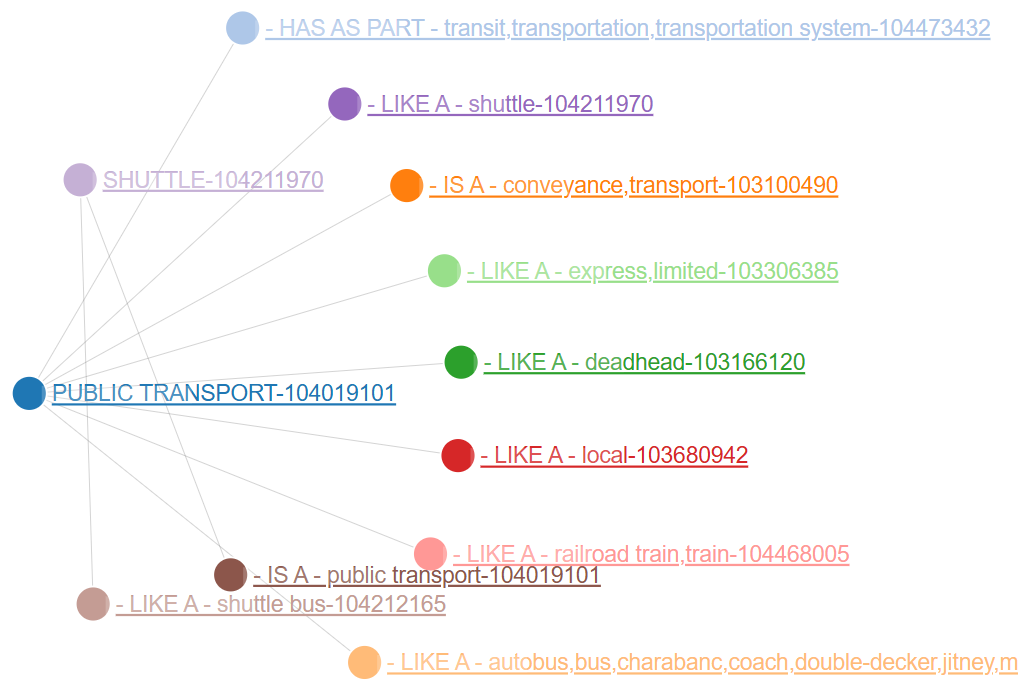
\includegraphics[width=0.6\textwidth]{rysunki/heurystyka_transport_publiczny.png}
            \captionof{figure}{ Graf bazowy WordNet w języku angielskim dla wyrażenia \enquote{public transport} \cite{wordnet_d3} }
            \label{heurystyka_transport_publiczny}
        \end{center}
        
        Ponadto, doskonałym sposobem na analizowanie tekstu są wyrażenia regularne, inaczej zwane regeksami (ang. \textit{regex}). Regeks jest sekwencją znaków, która definiuje wzorzec stosowany do dopasowania i szukania słów w tekście. Wyrażenia regularne stosowane są po to, aby dodawać do systemu wiedzę z konkretnego zakresu. Dobrym przykładem użycia wyrażeń regularnych będzie program, który na podstawie numeru kierunkowego określa, czy dzwoniący klient pochodzi z Polski czy z zagranicy, aby w razie potrzeby zestawić połączenie z konsultantem mówiącym w języku angielskim. Regeksy można podzielić na: 
        
        \begin{itemize}
            \item probabilistyczne — określają prawdopodobieństwo dopasowania szukanego słowa do wzorca,
            \item deterministyczne — określają zero-jedynkowo czy szukane słowo pasuje do wzorca.
        \end{itemize}

        Innym przydatnym narzędziem, używanym do modelowania języka naturalnego, jest gramatyka bezkontekstowa (ang. \textit{context-free grammar} — CFG). Wykorzystuje się ją do znacznie głębszej analizy niż wyżej opisany regeks. Jak trafnie opisano w książce \cite{sowmya_ksiazka_nlp2023}, \enquote{CFG można wykorzystać do wyodrębniania bardziej skomplikowanych, hierarchicznych informacji, które mogłyby umknąć wyrażeniu regularnemu}. Formalnie CFG definiowana jest jako czwórka $G=(N,T,P,S)$, gdzie $N$ jest zbiorem nieterminali, $T$ jest alfabetem terminalnym, $P$ jest zbiorem reguł w postaci $A \rightarrow \alpha$, a $S$ stanowi symbol początkowy gramatyki. Język generowany przez $G$, oznaczany jako $L(G)$, jest zbiorem słów nad alfabetem $T$ osiągalnych z symbolu startowego $S$ i stosujących reguły gramatyki $P$.


        \subsection{Metody reprezentacji tekstu}
        W nowoczesnych systemach przetwarzania języka naturalnego, oprogramowanie dokonuje segmentacji tekstu na zdania i słowa. Tak wydzielone struktury danych definiuje się jako tokeny. W zależności od rodzaju segmentacji, technikę tę nazywa się tokenizacją zdaniową lub wyrazową. Jak trafnie podają autorzy książki \cite{zaawansowane_techniki_NLP2025}, \enquote{proces tokenizacji jest ważnym wstępnym etapem w wielu zadaniach NLP, ponieważ przekształca on nieustrukturyzowane dane tekstowe w ustrukturyzowany format, który można analizować z użyciem algorytmów uczenia maszynowego lub innych technik}. Na poniższym rysunku \ref{nltk_tokenizer} zaprezentowano przykład tokenizacji wyrazowej z wykorzystaniem biblioteki Natural Language Tool Kit (NLTK).

        \begin{center}
            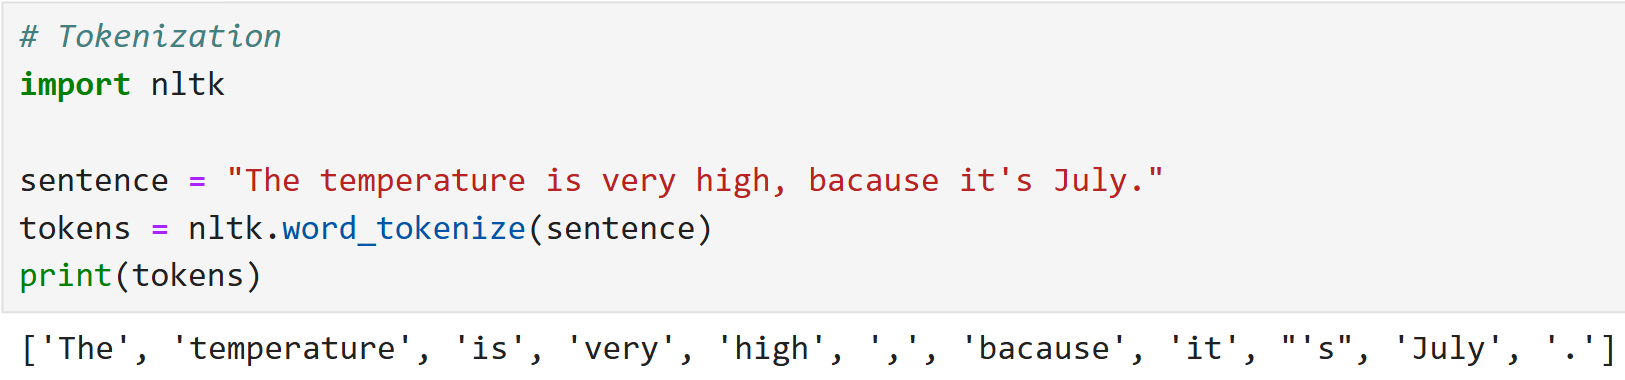
\includegraphics[width=0.8\textwidth]{rysunki/nltk_tokenizer.png}
            \captionof{figure}{ Przykład tokenizacji wyrazowej wykonanej przy użyciu biblioteki NLTK \cite{nltk_tokenization_library}}
            \label{nltk_tokenizer}
        \end{center}

        \noindent Kolejnymi ważnymi zagadnieniami w kontekście wstępnego przetwarzania tekstu są lematyzacja (ang. \textit{lemmatization}) oraz tematyzacja (ang. \textit{stemming}). Pierwszy termin odnosi się do uproszczenia słowa do jego postaci podstawowej lub słownikowej, nazywanej lematem. Pozwala to na traktowanie słowa jako znormalizowany wyraz. Drugi termin dotyczy redukcji słów do formy pozbawionej końcówek, nazywanej tematem. Celem tego zabiegu jest ujednolicenie różnych odmian i wariantów wyrazu poprzez przypisanie ich do wspólnej formy podstawowej. Na rysunku \ref{nltk_lem_stem} przedstawiono przykłady obydwu tych zagadnień z wykorzystaniem biblioteki NLTK.

       \begin{center}
            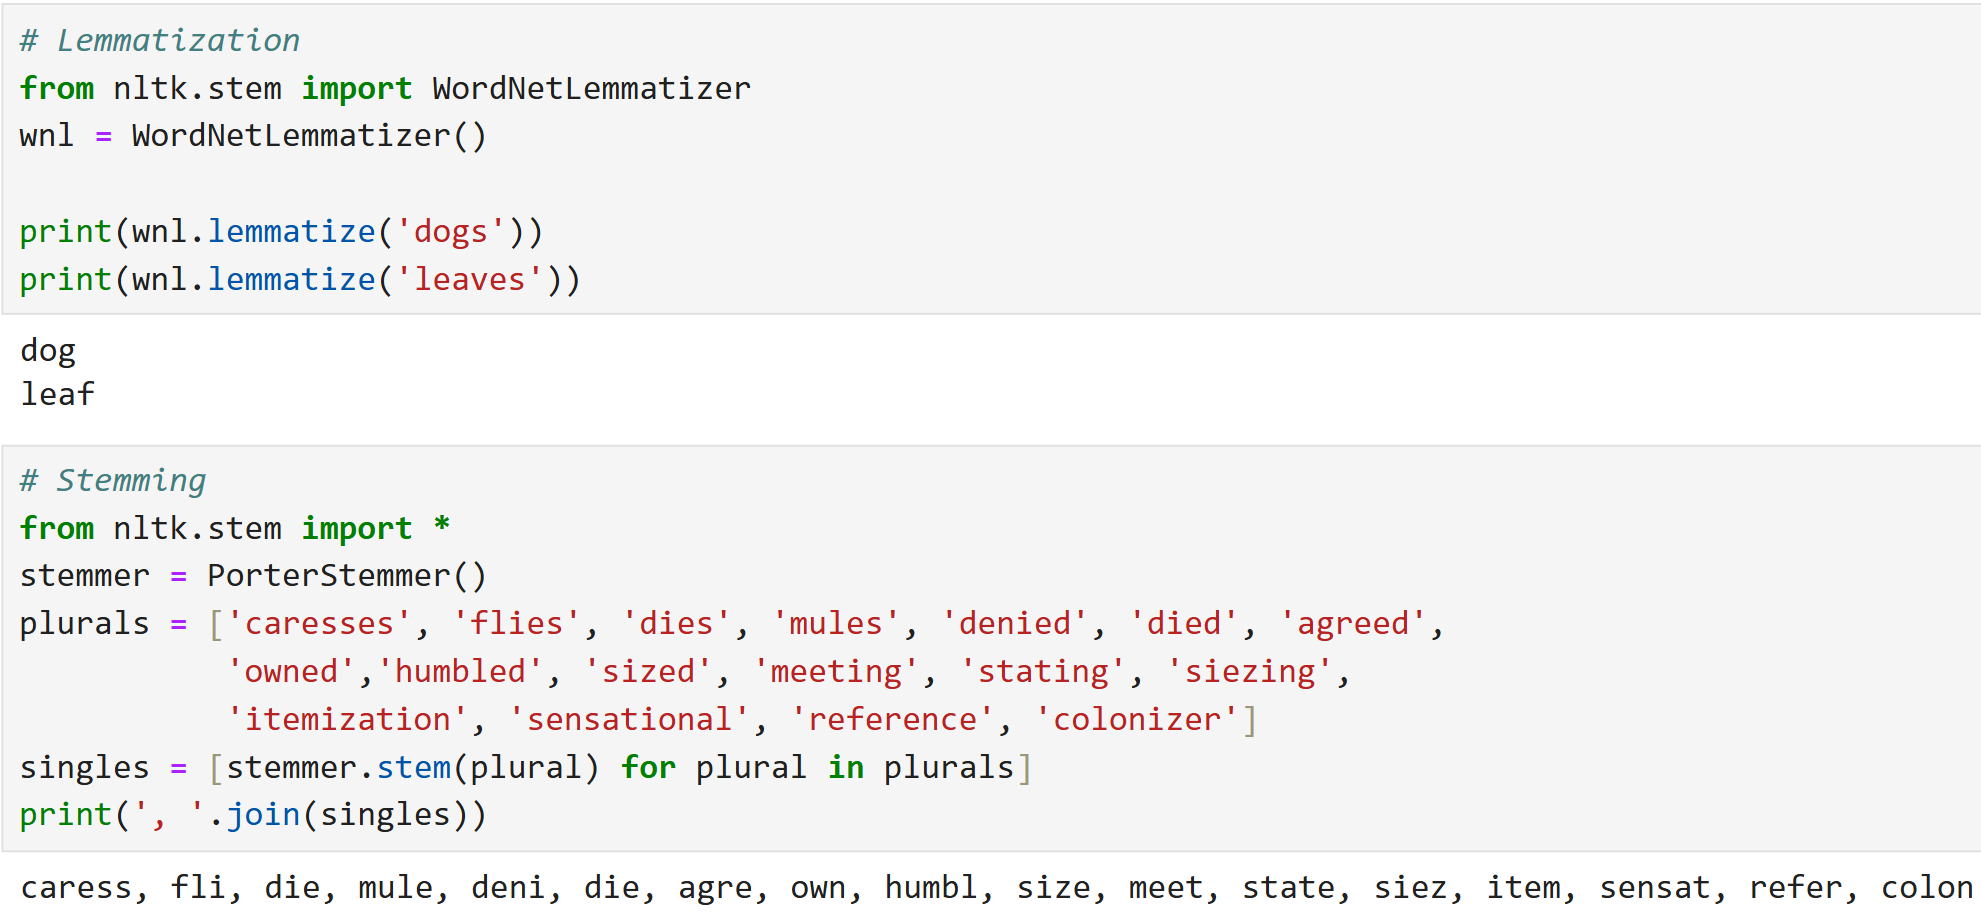
\includegraphics[width=0.85\textwidth]{rysunki/nltk_lem_stem.png}
            \captionof{figure}{ Przykład lematyzacji i tematyzacji wykonanych przy użyciu biblioteki NLTK \cite{nltk_tokenization_library}}
            \label{nltk_lem_stem}
        \end{center}

        Po wstępnym przygotowaniu tekstu następuje proces reprezentacji, który jest szczególnie ważny w kontekście uczenia maszynowego. Do klasycznych i najbardziej popularnych metod zalicza się: 

        \begin{itemize}
            \item worek słów (ang. \textit{bag of words} — BoW) — prosta i powszechnie stosowana metoda konwersji ciągu wyrazów na wektor liczb, które określają częstotliwości występowania przetwarzanych słów, zważając na kolejność ich występowania i kontekst,
            \item worek n-gramów — uogólniona funkcjonalność BoW uwzględniająca kolejność występujących słów w sekwencji,
            \item TF-IDF — technika ilustrująca ważność słów w bloku tekstowym, uwzględniająca nie tylko częstotliwość, lecz także rzadkość ich występowania,
            \item word2vec — technika posiadająca architekturę CBOW lub skip-gram, umożliwiająca tworzenie wielowymiarowych wektorowych reprezentacji słów, inaczej zwanych osadzeniami (ang. \textit{embeddings}) oddającymi znaczenia wyrażeń i ich wzajemne relacje.
        \end{itemize}

        
        \subsection{Uczenie maszynowe w NLP}
        Uczenie maszynowe (ang. \textit{machine learning} — ML) jest poddziedziną sztucznej inteligencji, którą współtworzą trzy główne dziedziny: informatyka, robotyka i statystyka. Są to odpowiednio zaprogramowane algorytmy potrafiące się doskonalić (uczyć) z danych bez ingerencji programisty. Jak trafnie opisano w lekturze \cite{sowmya_ksiazka_nlp2023} \enquote{każde podejście do NLP oparte na uczeniu maszynowym, nadzorowanym czy nie, zwykle składa się z trzech etapów: ekstrakcja cech z tekstu, użycie reprezentacji cech do uczenia modelu oraz ocenianie i ulepszanie modelu}.
        
        Pierwszym wartym uwagi algorytmem jest naiwny klasyfikator bayesowski (ang. \textit{naive bayes classifier}). To bardzo szybkie i łatwe w użyciu podejście jest powszechnie stosowane do wstępnego klasyfikowania tekstów. 
        Na przykład, przy filtrowaniu wiadomości e-maili, jeżeli algorytm wykrył w temacie słowo \enquote{wygrana}, którego występowanie w 90\% przypadków wskazuje na spam, to wiadomość zostanie zaklasyfikowana do tej kategorii. Jak wskazuje nazwa algorytmu, opiera się on na twierdzeniu Bayesa. Twierdzenie to opisano wzorem \ref{wzór_bayesa}, który określa prawdopodobieństwo wystąpienia klasy decyzyjnej $y$, pod warunkiem wystąpienia wektora atrybutów $x$. 

        \begin{equation}
        \begin{aligned}
            P(Y = y | X = x) = \frac{P(X = x | Y = y) P(Y = y)}{P(X = x)}
        \end{aligned}
        \label{wzór_bayesa}
        \end{equation}
        
        Drugim klasycznym podejściem w NLP jest maszyna wektorów nośnych (ang. \textit{support vector machine — SVM}). Algorytm ten może nauczyć się liniowej lub nieliniowej granicy decyzyjnej w celu oddzielenia danych (np. tekstów) należących do różnych klas, zachowując maksymalną odległość między nimi. Pomimo długiego czasu treningu, za sprawą dużej odporności na szumy i zmienność w danych, SVM jest jednym z najskuteczniejszych algorytmów. Na poniższej ilustracji \ref{svm} przedstawiono przykład użycia SVM.

        \begin{center}
            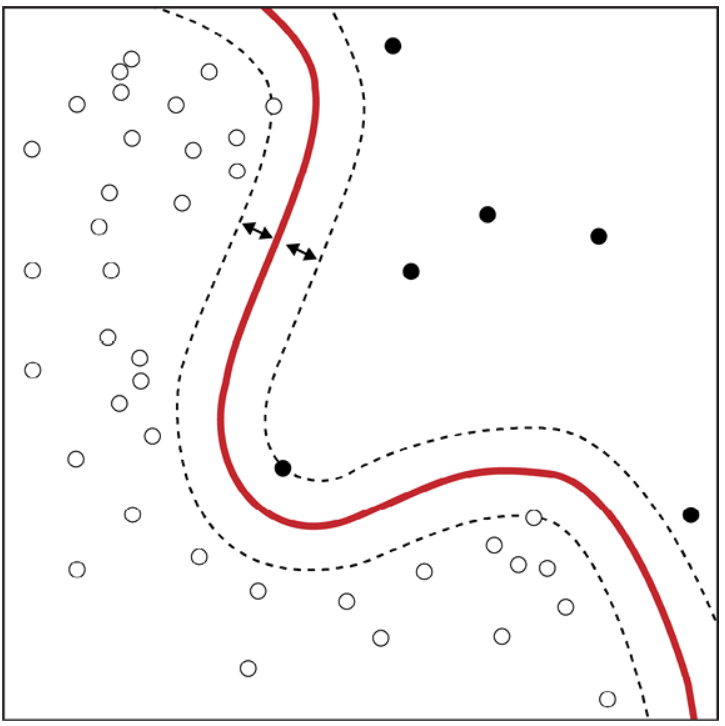
\includegraphics[width=0.4\textwidth]{rysunki/svm.png}
            \captionof{figure}{ Przykład zastosowania SVM dla dwuwymiarowej przestrzeni cech \cite{sowmya_ksiazka_nlp2023}}
            \label{svm}
        \end{center}
        
        
        \subsection{Uczenie głębokie w NLP}
        W ubiegłych latach dużą popularność zyskały głębokie sieci neuronowe, które stanowią fundament uczenia głębokiego (ang. \textit{deep learning}), poddziedziny uczenia maszynowego. Doskonale potrafią uczyć się skomplikowanych i nieustrukturyzowanych form danych, jak język naturalny.
        
        Na pierwszy plan wysuwają się rekurencyjne sieci neuronowe (ang. \textit{recurrent neural network} — RNN). Algorytm ten definiuje się jako model, który wytrenowany na danych sekwencyjnych lub czasowych (np. tekst lub mowa) potrafi dokonywać sukcesywnych predykcji czy wniosków, bazując na sekwencyjnym wejściu. Na rysunku \ref{rnn} zaprezentowano schemat działania RNN na przykładzie danych tekstowych.

        \begin{center}
            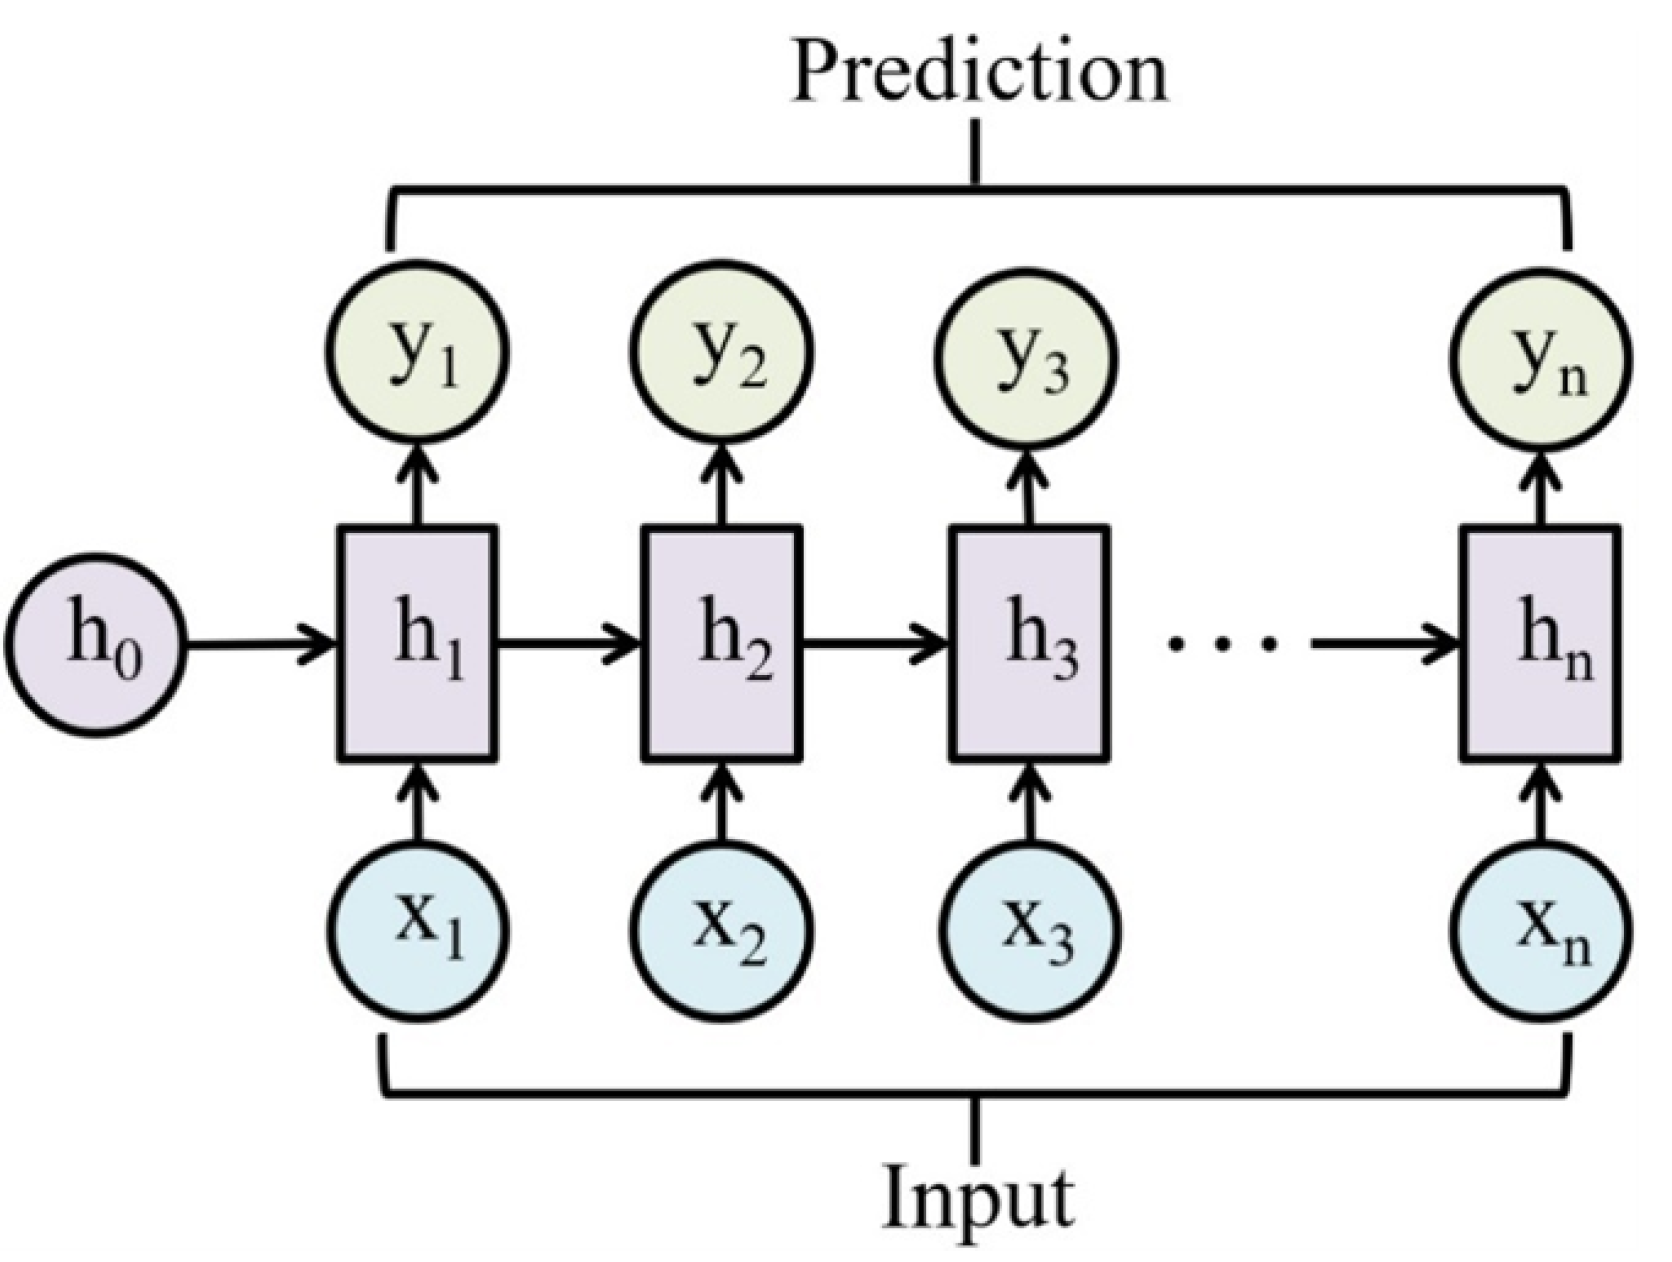
\includegraphics[width=0.5\textwidth]{rysunki/rnn.png}
            \captionof{figure}{ Schemat rekurencyjnej sieci neuronowej \cite{rnn_article2024}} 
            \label{rnn}
        \end{center}

        \noindent Istotnym wariantem rekurencyjnych sieci neuronowych, który sprawia, że  przestają one być \enquote{zapominalskie}, jest długa pamięć krótkotrwała (ang. \textit{long short-term memory} — LSTM). Sieci uczą się i zapamiętują długie sekwencje danych poprzez stan komórki (ang. \textit{cell state}) odzwierciedlający magistralę danych, której zawartość jest wybiórczo aktualizowana lub usuwana przez matematyczne mechanizmy bramek.

       Drugim kluczowym podejściem są konwolucyjne sieci neuronowe (ang. \textit{convolutional neural network} — CNN), które często wykorzystuje się w wizji komputerowej. Każde słowo w zdaniu może być zastąpione przez wektor słowa, a każdy z wektorów ma ten sam rozmiar. Taka struktura pomaga na ich pionowe zestawienie tworząc macierz o wymiarach $h \times w$, gdzie $h$ jest liczbą słów w zdaniu, a $w$ długością wektorów. Dane przygotowane w ten sposób przypominają strukturę obrazu, co umożliwia ich skuteczne przetwarzanie za pomocą CNN.
\cleardoublepage

\chapter{Rozpoznanie dużych modeli językowych}
W niniejszym rozdziale autor przybliżył dziedziny, w których generatywna sztuczna inteligencja może wspomagać ludzką kreatywność, zapewniając przy tym oszczędność czasu. Dodatkowo, opisał skomplikowaną architekturę transformer, która stanowi podstawę działania dużych modeli językowych. One także zostały dokładnie i praktycznie opisane w ostatnim podrozdziale.


    \section{Generatywna sztuczna inteligencja}
    Termin \enquote{generatywna sztuczna inteligencja} (ang. \textit{generative artificial intelligence} — GenAI) nie schodzi z ust ludzi na całym świecie od 30 listopada 2022. Tego dnia opublikowano chatbota ChatGPT, który zrewolucjonizował formę kreatywnej komunikacji człowiek-komputer. Modele generatywne nie tylko zaczęły tworzyć tekst na zaawansowanym poziomie, ale także obrazy, muzykę, filmy czy oprogramowanie. Jak słusznie opisano w książce \cite{genAI_langchain2024} \enquote{te modele mogą zapewnić bardzo wiele funkcjonalności, między innymi wyszukiwanie semantyczne, manipulowanie zawartością oraz klasyfikację}. Dzięki tym rozwiązaniom, wykorzystując automatyzację, łatwo zredukowano koszty, a ludzka kreatywność wzrosła do niespotykanego dotąd stopnia.
        

        \subsection{Generowanie tekstu}
        Jednym z najczęstszych zastosowań GenAI jest tworzenie nowych treści w języku naturalnym. Modele takie jak GPT-4, opracowany przez amerykańską firmę OpenAI, mogą być wykorzystywane do streszczania długich treści, pisania artykułów czy rozwiązywania równań matematycznych z pełnym opisem toku rozumowania. Wytrenowane na ogromnych zbiorach tekstu, posługują się średnio ponad osiemdziesięcioma językami, co czyni je perfekcyjnymi tłumaczami.
        
        
        \subsection{Generowanie obrazu}
        W 2014 roku Ian Goodfellow zdefiniował architekturę sieci Generative Adversarial Network (GAN) służącej do generowania realistycznych obrazów. W praktyce niemal niemożliwe jest odróżnienie obrazu wygenerowanego od rzeczywistego. W 2021 roku firma OpenAI wdrożyła DALL-E — nowy i innowacyjny generatywny model. W przeciwieństwie do poprzedniej architektury, ta umożliwiła tworzenie obrazów na podstawie tekstu w języku naturalnym (ang. \textit{text-to-image}). Generowanie obrazu umożliwia poszerzanie zbiorów treningowych (augmentację danych) dla wizji komputerowej, tworzenie bardziej kreatywnych grafik w marketingu czy projektowanie nowych produktów cyfrowych.
        
        
        \subsection{Generowanie muzyki}
        Illiac Suite jest pierwszym utworem muzycznym w pełni skomponowanym przez sztuczną inteligencję. Jego pomysłodawcami byli Lejaren Hiller i Leaonardo Isaacson w 1957 roku. Od tamtej pory bez przerwy rozwijano techniki generowania muzyki. W 2016 roku firma Google zaprezentowała otwartoźródłowy projekt badawczy Magenta. Wykorzystano w nim głównie rekurencyjne sieci neuronowe. Cztery lata później OpenAI zaprezentowało Jukebox \cite{dhariwal2020jukebox}. Jest to sieć neuronowa generująca muzykę, dzięki której użytkownik posiada kontrolę nad gatunkiem, głosem artysty oraz stylem muzycznym utworu.

        
        \subsection{Generowanie wideo}
        Rozwój powyższych trzech dziedzin generowania treści w ostatnich latach przyczynił się do zaawansowanego rozwoju generowania wideo. Na dzień dzisiejszy, do najpopularniejszych rozwiązań zalicza się Runway Gen-4.5, OpenAI Sora oraz Google Veo. Każde z nich umożliwia tworzenie realistycznych lub stylizowanych materiałów wideo na podstawie obrazów lub zapytania tekstowego. Przytoczone oprogramowania najlepiej radzą sobie przy tworzeniu krótkich, kilkuminutowych treści. Z jednej strony technologia ta otwiera szereg nowych możliwości w pracy artystów czy twórców internetowych. Z drugiej zaś strony, za pomocą fałszywych treści wideo (ang. \textit{deepfake}) coraz częściej dochodzi do manipulacji społeczeństwa na platformach społecznościowych i w mediach.

        
        \subsection{Wpływ na środowisko}
        W celu obsługi i rozwijania modeli generatywnych na szeroką skalę, wymagana jest ogromna moc obliczeniowa. Wytrenowanie pojedynczego modelu potrafi zużyć nawet 50 GWh energii. Dzieje się tak, ponieważ wymagane jest do tego wykorzystanie tysięcy procesorów graficznych (ang. \textit{graphics processing unit} — GPU), wykonujących obliczenia przez wiele tygodni. Utrzymanie infrastruktury, w tym odpowiadanie na zapytania (prompty), kiedy model generatywny jest wdrożony na rynek, także kosztuje olbrzymią ilość energii każdego dnia.

        
        \subsection{Prawa autorskie}
        Relacja między GenAI a prawem jest wciąż dynamicznie kształtowana. Obecnie, zgodnie z obowiązującym prawem w Polsce i UE, tylko człowiek może być autorem wszelkich treści kreatywnych. Jeżeli coś zostało automatycznie wygenerowane przez sztuczną inteligencję, bez zasadniczego wkładu intelektualnego człowieka, nie podlega to ochronie praw autorskich.

        
        \subsection{Ogólna sztuczna inteligencja}
        Ogólna sztuczna inteligencja (ang. \textit{artificial general intelligence} — AGI) jest koncepcją rozwoju sztucznej inteligencji do poziomu ogólnej adaptacji i zdolności do absorbowania wiedzy z różnych dziedzin. W swoim zamyśle, AGI osiągnie poziom inteligencji zbliżony do ludzkiego. Jak trafnie opisał autor artykułu \cite{agi2014}, system wykazujący się ogólną sztuczną inteligencją powinien generalizować wiedzę, co umożliwi jej transferowanie między różnymi problemami i kontekstami.

        
    \section{Architektura transformer}
    Problemem tradycyjnych modeli takich jak RNN, LSTM czy GRU, przetwarzających dane sekwencyjnie, jest gubienie kontekstu dłuższych treści. Reprezentacja każdego tokena zależy od poprzednich tokenów z ciągu oraz od niego samego, ograniczając szybkość i wydajność rozwiązania. Jednakże, w 2017 roku firma Google zaprezentowała artykuł \enquote{Attention is all you need} \cite{attention_is_all_you_need2017}, w którym przedstawiono architekturę transformer. Rozwiązanie to nie wykorzystuje złożonych konwolucyjnych czy rekurencyjnych sieci neuronowych, znosząc konieczność przetwarzania sekwencyjnego. Transformer bazuje na mechanizmie samouwagi, inaczej zwanym atencją ze skalowalnym iloczynem skalarnym. Umożliwia to równoległe przetwarzanie danych, wychwytując relacje między bardzo odległymi elementami w sekwencji. Pełny schemat architektury przedstawiono na rysunku \ref{transformer}.

    \begin{center}
        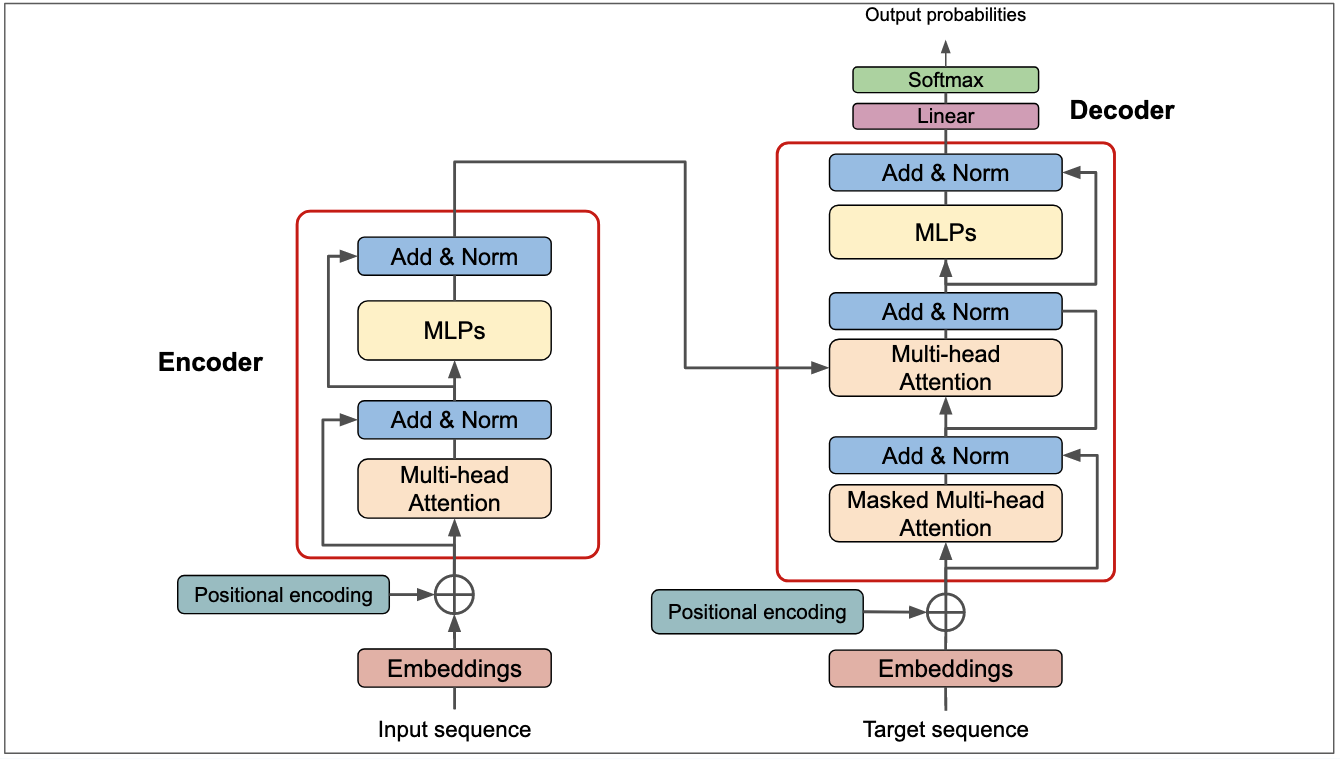
\includegraphics[width=0.75\textwidth]{rysunki/transformer.png}
        \captionof{figure}{ Architektura transformera \cite{attention_is_all_you_need2017}} 
        \label{transformer}
    \end{center}


        \subsection{Tokenizacja}
        Tokenizacja oznacza zamianę tekstu (słów, podwyrazów lub znaków) na wartości liczbowe (tokeny), które są zrozumiałe dla modelu. Jest to pierwszy i najbardziej kluczowy krok, ponieważ sieci neuronowe operują wyłącznie na liczbach i w nich kryje się znaczenie poszczególnych tokenów. Poniżej przedstawiono przykład konwersji tekstu na tokeny wraz z ich numerycznymi identyfikatorami \ref{llm_tokenizer}.

        \begin{center}
            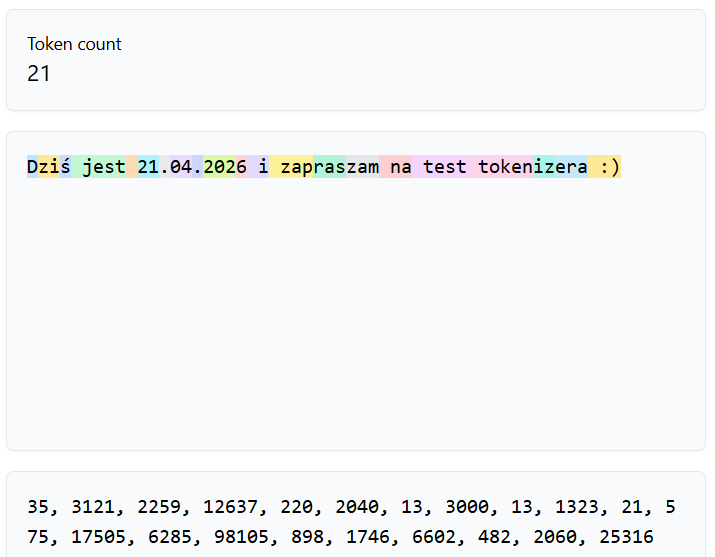
\includegraphics[width=0.5\textwidth]{rysunki/llm_tokenizer.png}
            \captionof{figure}{ Przykład tokenizacji tekstu \cite{tiktokenizer}} 
            \label{llm_tokenizer}
        \end{center}


        \subsection{Reprezentacja wektorowa}
        W następnym kroku, numeryczne identyfikatory tokenów, które są liczbami całkowitymi, przekształcane są w wielowymiarowe wektory liczb rzeczywistych. Tak reprezentowane słowa umiejscowione są w przestrzeni wielowymiarowej, gdzie odległość między wektorami odwzorowuje podobieństwo semantyczne między słowami – im bardziej podobne znaczenia wyrazów, tym bliżej siebie się znajdują. Tę operację nazywa się osadzeniem (ang. \textit{embedding}).
        
        
        \subsection{Kodowanie pozycyjne}
        W transformerze nie ma domyślnie wbudowanej funkcjonalności rozpoznawania kolejności przetwarzanych słów. Odpowiedź na ten problem stanowi kodowanie pozycyjne (ang. \textit{positional encoding}). Jest to technika, która umożliwia podanie do transformera informacji dotyczącej pozycji tokenów w sekwencji. Polega na tym, że do każdego wektora embeddingu dodawany jest wektor jego pozycji.
        
        
        \subsection{Mechanizm samouwagi}
        Mechanizm samouwagi (ang. \textit{self-attention mechanism}) umożliwia modelowi analizowanie różnych fragmentów na raz, zamiast przetwarzać dane wejściowe w kolejności. Algorytm wylicza wagi uwagi określające względną ważność każdej części tekstu w sekwencji. Następnie stosuje te wagi, aby zmniejszyć lub zwiększyć wpływ analizowanych fragmentów na predykcję transformera.

        
        \subsection{Koder i dekoder}
        Zadaniem kodera (ang. \textit{encoder}) jest pobranie sekwencji danych na wejściu i generowanie sekwencji stanów ukrytych, z których każdy jest sumą ważoną wszystkich operacji osadzenia (embeddingu) danych wejściowych. Z kolei dekoder (ang. \textit{decoder}), otrzymując sekwencję danych wyjściowych, przesuniętą w prawo o jedną pozycję, generuje sekwencję estymacji. Każda z nich jest sumą ważoną stanów ukrytych kodera, zależną od poprzedniego stanu dekodera \cite{llm_w_proj_oprogramowania2024}. Na końcu dekodera dochodzi do konwersji surowych wartości mechanizmu uwagi (tzw. logitów) na rozkład prawdopodobieństwa możliwych odpowiedzi (tokenów). Odbywa się to za pomocą funkcji softmax.
        
    
    \section{Definicja dużego modelu językowego}
    Dużym modelem językowym (ang. \textit{large language model} — LLM) nazywamy algorytm oparty na uczeniu głębokim, który posiada miliardy wewnętrznych parametrów (wag) i został wytrenowany na gigantycznych zbiorach danych. Zbudowany jest na podstawie zdefiniowanej wyżej architektury transformer. Model stworzony został do wykonywania wielu zadań związanych z przetwarzaniem języka naturalnego, takich jak generowanie, tłumaczenie czy podsumowywanie tekstu \cite{llm_w_proj_oprogramowania2024}. Warto podkreślić, iż duże modele językowe nie \enquote{myślą} w sensie ludzkim, lecz estymują kolejny najbardziej prawdopodobny token w oparciu o tekst na wejściu. Są one dostępne dla szerokiego grona odbiorców dzięki dedykowanym interfejsom użytkownika (chatbotom) oraz API. Specyfikę najpopularniejszych z nich przybliżono w poniższym podrozdziale.

    
        \subsection{Przegląd popularnych dużych modeli językowych}
        Pierwszym rozpatrywanym dużym modelem językowym jest Generative Pre-trained Transformer (GPT). Został stworzony przez założoną w 2015 roku amerykańską firmę OpenAI, która obecnie jest liderem w dziedzinie generatywnej sztucznej inteligencji. Model GPT jest wstępnie wytrenowany (ang. \textit{pre-trained}) na ogromnych zbiorach nieetykietowanych danych, dzięki czemu nabywa ogólne zdolności językowe i staje się wszechstronną bazą, która posiada możliwość dostrojenia do konkretnych zadań. Pierwszym produktem firmy, wykorzystującym architekturę transformer, był GPT-1 stworzony w 2018 roku. Sukces rodziny modeli GPT, szczególnie od 2022 roku za sprawą wydania aplikacji ChatGPT bazującej na modelu GPT-3.5, stał się katalizatorem, który zmusił konkurencję do zintensyfikowania prac nad własnymi rozwiązaniami AI. Nowsze modele, na przykład GPT-4o, nie tylko przetwarzają tekst, ale także dźwięk i obraz.

        Założona w 2023 roku chińska firma Hangzhou DeepSeek Artificial Intelligence Basic Technology Research w 2025 roku wdrożyła na rynek porównywalnego chatbota DeepSeek. Wykorzystywał znacznie tańszy otwartoźródłowy model DeepSeek-R1 o osiągach porównywalnych do GPT-4, co stanowiło ogromną konkurencję dla produktów firmy OpenAI. Co więcej, chińske przedsiębiorstwo przyznało, że trening ich modelu był kilkanaście razy tańszy i zużywał do dziesięciu razy mniej mocy obliczeniowej niż konkurencyjne modele. Poza podstawową architekturą transformer, modele DeepSeek wykorzystują dwa dodatkowe podejścia w celu poprawy ich wydajności — strategię trenowania modelu wolną od strat pomocniczych (ang. \textit{auxiliary-loss-free strategy}) oraz strategię celu treningowego polegającego na przewidywaniu wielu tokenów jednocześnie \cite{deepseek_technical_report2024}.

        Trzecim prezentowanym modelem jest Gemini od amerykańskiej firmy Google, wcześniej znanym pod nazwą Bard. Jako pierwszy, w 2023 roku, zadebiutował wariant Gemini 1.0. Rodzina modeli od Google także bazuje na architekturze transformer. Natomiast, spośród reszty dostępnych modeli, w momencie publikacji Gemini wyróżnił się multimodalnością. Został natywnie zaprojektowany do przetwarzania tekstu, audio, obrazu i wideo na jednym strumieniu danych.

        Claude 1, czyli pierwszy model amerykańskiego przedsiębiorstwa Anthropic, także miał swoją premierę w 2023 roku. Na ten moment, modele rodziny Claude można podzielić na trzy kategorie od najmniej do najbardziej zaawansowanej: Haiku, Sonnet i Opus. Są one najlepszymi modelami na rynku w kontekście analizy i generowania kodu. Modele Claude są trenowane w ramach strategii Constitutional AI, polegającej na dostosowaniu systemów sztucznej inteligencji do ludzkich wartości, czyniąc je pomocnymi, nieszkodliwymi i szczerymi \cite{constitutional_ai2022}.
        
        Ostatnim wartym uwagi modelem jest Grok, stworzony przez amerykańską firmę xAI. Pierwszym ich produktem był Grok-1, wydany w 2023 roku. Poprzez integrację z platformą X, Grok ma aktualną wiedzę dotyczącą bieżących informacji ze świata i trendów. W momencie gdy inne modele dążą do bycia neutralnymi i uprzejmymi w swoich wypowiedziach, Grok jest mniej ocenzurowany, co wpływa na jego skłonności do sarkazmu i bycia bezpośrednim. Jest skłonny do generowania kontrowersyjnych wypowiedzi dotyczących historii, teorii spiskowych, polityki oraz sfery seksualnej.


        \subsection{Ograniczenia modeli LLM}
        Chociaż duże modele językowe są niezwykle popularne i często zaskakująco trafne w swoich wypowiedziach, mają one ograniczenia i niedoskonałości. Poniżej opisano czynniki wpływające na to, że LLMy nie są nieomylne i zawsze jako użytkownicy powinniśmy weryfikować ich wypowiedzi. Warto rozumieć te ograniczenia, aby móc świadomie i skutecznie tworzyć aplikacje bazujące na modelach językowych. Problemy te dowodzą, że ludzka inteligencja i twórczość są niezastąpione.

        Pierwszym czynnikiem ograniczającym skuteczność wypowiedzi w wielu modelach językowych jest nieaktualny stan wiedzy. Jak trafnie opisano w książce \cite{genAI_langchain2024}, \enquote{modele LLM polegają jedynie na danych treningowych, bez integracji z zewnętrznym źródłem danych nie mogą dostarczać aktualnych informacji ze świata}.

        Drugim istotnym powodem, który powinien wzbudzać ograniczone zaufanie jest niedeterministyczne zachowanie. LLMy mogą generować różne, a czasem nawet sprzeczne odpowiedzi na to samo zapytanie (prompt). Wynika to z ich probabilistycznej natury — wyniki zależą od rozkładu prawdopodobieństwa, a nie od sztywno zdefiniowanych reguł. Modele potrafią generować nieprawidłowe lub bezsensowne informacje, ponieważ polegają na wyuczonych wzorcach, a nie na dokładności faktów. Takie zjawisko nazywa się halucynacją.
        
        Kolejnym ważnym aspektem są tendencje modeli do pewnych zachowań czy stronniczości ideologicznych wynikające z danych treningowych. LLMy mogą mieć podłoże religijne, być z natury upolitycznione lub generować treści o charakterze dyskryminacyjnym. Ponadto, przez brak weryfikacji, zbiory danych mogą zawierać fałszywe informacje i szkodliwe porady, które model traktuje jako wzorce do naśladowania.
        
        Inną trudnością jest przyjmowanie właściwego kontekstu przez LLMy. Użytkownik często zakłada, że model \enquote{domyśli się} kim jest, jakie są jego prawdziwe intencje oraz jakie jest tło opisywanej sytuacji. W rzeczywistości, poza promptem, model nie ma innego punktu odniesienia, aby zapewnić nam precyzyjną i rzetelną odpowiedź w złożonych okolicznościach. Dodatkowo, modele językowe mają tendencję do zapominania kontekstu. Mogą one nie pamiętać podanych wcześniej szczegółów w bieżącej czy innej konwersacji.


        \subsection{Dostrajanie modelu}
        Dostrajanie (ang. \textit{fine-tuning}) przeprowadza się na wcześniej wytrenowanym dużym modelu językowym. Ten proces polega na dodatkowym treningu algorytmu na znacznie mniejszym, specyficznym zbiorze danych. Działanie to ma na celu poszerzenie wewnętrznego stanu wiedzy i udoskonalenie modelu do wykonywania dedykowanych zadań \cite{fine_tuning2024}.
\cleardoublepage

\chapter{Wprowadzenie do generowania wspomaganego wyszukiwaniem}
W celu zapewnienia modelowi aktualnego stanu wiedzy lub dostępu do naszych prywatnych zasobów danych istnieje znacznie bardziej wydajne podejście niż fine-tuning. Chodzi o technikę RAG, którą ze szczegółami przybliżono w niniejszym rozdziale. Dodatkowo, autor pochylił się nad definicją agentów AI, które w doskonały sposób implementują tę technikę. 


    \section{Definicja techniki RAG}
    Generowanie wspomagane wyszukiwaniem (ang. \textit{retrieval-augmented generation} — RAG) jest techniką umożliwiającą dużym modelom językowym pozyskiwanie i przetwarzanie nowych informacji z zewnętrznych źródeł danych bez konieczności modyfikowania tych modeli. Pozwala to chatbotom zredukować halucynacje i zapewnić bardziej dokładne odpowiedzi na pytania dotyczące źródeł danych, na których model nie został wytrenowany. Mogą to być dane zarówno ustrukturyzowane jak i nieustrukturyzowane, takie jak: bazy danych SQL, prywatne pliki PDF, strony internetowe czy repozytoria kodu. Dzięki temu rozwiązaniu, można zapewnić chatbotom stały dostęp do aktualnej wiedzy ze świata, co pozwala zniwelować ograniczenia wynikające z daty zakończenia treningu modelu. Jedną z kluczowych zalet podejścia RAG jest zdolność LLMa do podawania źródeł danych, a nawet cytowania konkretnego fragmentu w swojej wypowiedzi. Pozwala to użytkownikom weryfikować informacje oraz zwiększyć zaufanie do generowanej przez model treści \cite{llm_for_production2024}. Na ilustracji \ref{rag} pokazano w uproszczeniu jak działa RAG.

    \begin{center}
        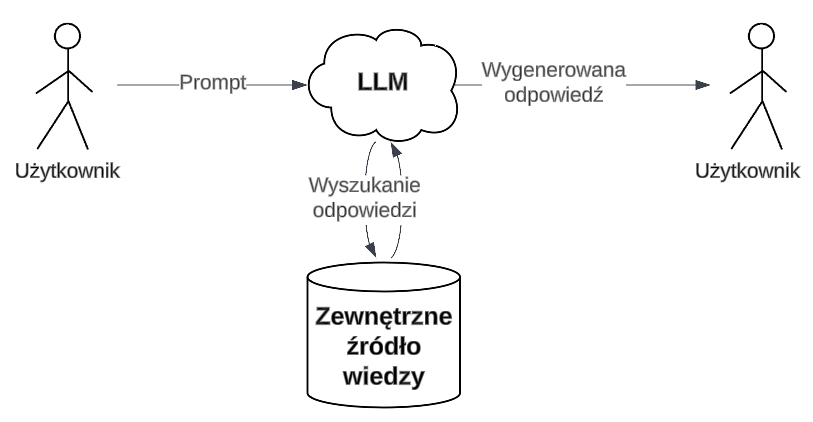
\includegraphics[width=0.6\textwidth]{rysunki/rag.png}
        \captionof{figure}{Uproszczony schemat generowania wspomaganego wyszukiwaniem}
        \label{rag}
    \end{center}
        
        
        \subsection{Embedder i wektorowa baza danych}
        Embedder przekształca zawartość źródła danych w reprezentację wektorową (embeddingi). Natomiast, wektorowa baza danych, która w większości przypadków stanowi zewnętrzne źródło wiedzy, przechowuje te embeddingi wraz z metadanymi dotyczącymi tekstów, obrazów czy audio. Pozwala to wnieść dodatkowy kontekst, czyli informacje z zewnętrznych źródeł danych do LLMa, który je wyszukuje na podstawie podobieństwa semantycznego do zapytania użytkownika. Warto nadmienić, że zawartość przetwarzanego dokumentu należy wpierw podzielić na wiele mniejszych porcji (ang. \textit{chunking}). Dodatkowo wyznacza się wspólne części kolejnych porcji tekstu (ang. \textit{overlapping}), w celu zachowania kontekstu między fragmentami. Standardowy rozmiar chunka wynosi od 256 do 512 tokenów, natomiast wartość overlapu zawiera się między 50 a 100 tokenów.
        
        
        \subsection{Wydobywanie informacji i generowanie odpowiedzi}
        Do szukania oraz pozyskiwania odpowiednich dokumentów i faktów z zewnętrznej bazy danych służy retriever. Podczas wydobywania informacji, nieustrukturyzowane zapytanie (prompt) użytkownika przekształcane jest na odpowiednią przestrzeń wektorową w celu odnalezienia istotnych informacji z bazy wektorowej. Następnie, generator analizuje pozyskaną treść i dopasowuje ją do zapytania użytkownika. Z wykorzystaniem dużego modelu językowego, tworzy odpowiedź w języku naturalnym uwzględniając wyekstrahowane fakty.


        \subsection{Porównanie RAG i fine-tuningu}
        Różnica między podejściem RAG i fine-tuning polega na tym, że te pierwsze poszerza wiedzę modelu \enquote{podłączając} go do własnej bazy danych, kiedy drugie wiąże się z kosztownym poszerzeniem wyuczonej już wiedzy modelu w konkretnej dziedzinie. Nie można jednogłośnie określić, które rozwiązanie jest lepsze, gdyż oba mają swoje zalety i wady, a dobór podejścia jest zależny od celu jaki chce się osiągnąć. RAG i fine-tuning nie wykluczają się wzajemnie, lecz mogą się uzupełniać, podnosząc wydajność modelu w określonych obszarach kompetencji modelu. W poniższej tabeli \ref{rag_vs_finetuning}, na podstawie artykułu \cite{rag_for_llm2023}, przedstawiono porównanie tych dwóch podejść.

        \begin{table}[h]
            \centering
            \caption{Zestawienie RAG i fine-tuningu \cite{rag_for_llm2023}}
            \begin{tabularx}{\textwidth}{|p{3.5cm}|X|X|}
            \hline
            \textbf{Porównywana cecha} & \textbf{RAG} & \textbf{Fine-tuning} \\
            \hline
            Aktualizacja wiedzy & Umożliwia bezpośrednią aktualizację bazy wiedzy, zapewniając stałą aktualność informacji bez konieczności dotrenowania modelu, co jest odpowiednie dla dynamicznie zmieniających się danych. & Statyczna wiedza modelu utrwalona w jego parametrach. Wymagane jest dotrenowanie w celu aktualizacji stanu wiedzy. \\ \hline
            
            Przetwarzanie danych & Wymaga minimalnego przetwarzania i przygotowania danych. & Polega na stworzeniu wysokiej jakości zbioru danych. Zbyt małe zbiory danych mogą nie przynieść znaczącej poprawy wydajności algorytmu. \\ \hline
            
            Interpretowalność & Wygenerowane odpowiedzi modelu można powiązać z konkretnymi źródłami danych. Zapewnia to wyższą interpretowalność i umożliwia ich łatwiejsze uzasadnienie. & Nigdy nie jest się pewnym dlaczego model odpowiedział w dany sposób i z jakiego źródła pochodzi jego odpowiedź, co utrudnia interpretowalność. \\ \hline
            
            Redukcja halucynacji & O wiele mniejsza szansa na halucynacje, gdyż odpowiedzi są oparte na zewnętrznych źródłach danych. & Pomaga zmniejszyć prawdopodobieństwo halucynacji poprzez trenowanie modelu na danych z konkretnej dziedziny. Natomiast, model nadal może wykazywać halucynacje przy napotkaniu nieznanych danych wejściowych. \\ \hline
            \end{tabularx}
            \label{rag_vs_finetuning}
        \end{table}


    \section{Agenty AI}
    Agentem AI (ang. \textit{AI agent}) nazywamy zaawansowany system, który autonomicznie postrzega swoje otoczenie i wykonuje określone zadania wykorzystując do tego zewnętrzne narzędzia (ang. \textit{external tools}), przy minimalnym nadzorze człowieka. Jego \enquote{mózgiem} jest duży model językowy. To dzięki niemu agent rozumie i wykonuje zadania zlecone przez użytkownika oraz stwierdza kiedy i jakiego zewnętrznego narzędzia użyć. Jak podaje artykuł \cite{ai_agents_that_matter2024}, im środowisko jest bardziej złożone — dynamiczne, składające się z wielu zadań czy o długim horyzoncie czasowym — tym bardziej system w nim operujący jest agentowy (ang. \textit{agentic}). Jednym z głównych celów wykorzystania agentów AI jest integracja z zewnętrznymi źródłami danych, co stanowi istotę podejścia RAG. Stają się one wtedy systemami łączącymi zdolność samodzielnego działania z dostępem do zewnętrznej wiedzy. Na poniższym rysunku \ref{ai_agent} zaprezentowano dobry przykład uproszczonego agenta AI stosującego RAG. Automatycznie sumuje ceny produktów znajdujących się w bazie SQL i wysyła maila z podsumowaniem na konkretny adres. System wykorzystuje do tego celu model językowy firmy OpenAI oraz odpowiednie narzędzia: narzędzie Postgres odpytujące bazę danych SQL, kalkulator i narzędzie wysyłające wiadomości z konta Gmail. Poniżej jest zaprezentowany przykładowy agent AI \ref{ai_agent}.

    \begin{center}
        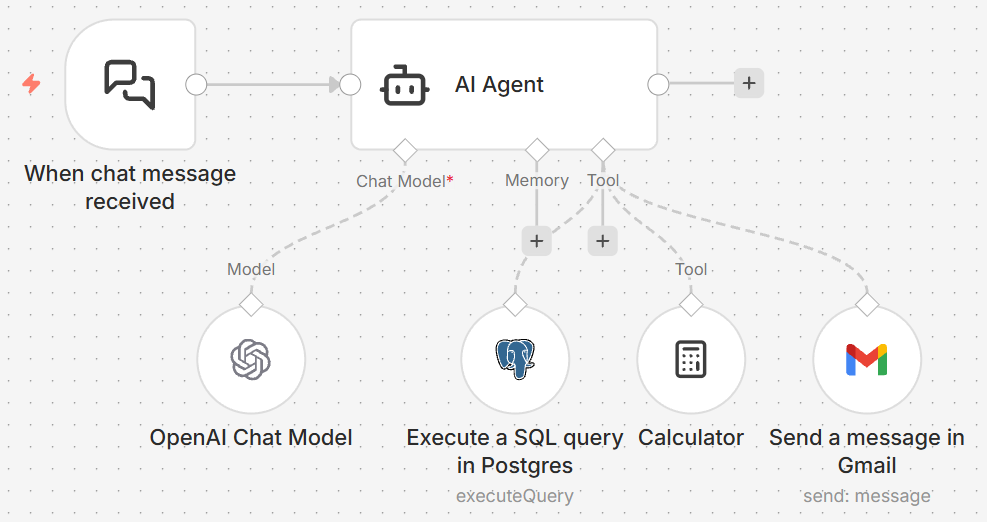
\includegraphics[width=0.65\textwidth]{rysunki/ai_agent.png}
        \captionof{figure}{ Przykład agenta AI wykorzystującego techniką RAG stworzonego z użyciem platformy n8n \cite{n8n}}
        \label{ai_agent}
    \end{center}


        \subsection{Prompt systemowy}
        Prompt systemowy (lub wiadomość systemowa) jest zbiorem instrukcji i kontekstu jaki podaje się do dużego modelu językowego, aby agent AI odpowiadał na pytania w pożądany przez nas sposób. Funkcja ta jest najczęściej wykorzystywana do: 
        \begin{itemize}
            \item ustawienia stylu i tonu odpowiedzi modelu,
            \item zdefiniowania roli i ograniczeń modelu,
            \item określenia kryteriów bezpieczeństwa i jakości podczas generowania odpowiedzi,
            \item wskazania formatu danych wyjściowych (na przykład JSON lub CSV).
        \end{itemize}

\cleardoublepage

\chapter{Przegląd literatury}
W tym rozdziale zaprezentowano przegląd trzech różnych artykułów naukowych, opisujących podejścia do testowania i ewaluacji dużych modeli językowych wykorzystywanych w systemach RAG. Pierwsze dwie publikacje oparte są na danych nieustrukturyzowanych, podczas gdy ostatnia skupia się na danych ustrukturyzowanych.
    

    \section{Benchmark MEBench}
    W artykule \enquote{MEBench: Benchmarking Large Language Models for Cross-Document Multi-Entity Question Answering} \cite{art1_2025} autorzy przedstawili MEBench, czyli skalowalny wielodokumentowy test wydajnościowy (ang. \textit{benchmark}). Zaprojektowany został do systematycznej ewaluacji systemów LLM zdolnych do wyszukiwania, łączenia informacji i wyciągania wniosków z rozproszonych i bogatych w treść zewnętrznych źródeł danych. Benchmark składa się z 4780 pytań podzielonych na trzy kategorie wnioskowania \ref{mebench_kategorie_pytan}: porównawcze, relacyjne i statystyczne. 

    \begin{table}[h]
        \centering
        \caption{ Definicja trzech kategorii pytań wchodzących w skład frameworka MEBench }
        \begin{tabularx}{\textwidth}{|p{5cm}|X|}
        \hline
        \textbf{Kategoria pytań} & \textbf{Definicja} \\
        \hline
        Wnioskowanie porównawcze & Umożliwia sprawdzenie czy LLM jest w stanie zestawić ze sobą elementy z różnorodnych źródeł danych zachowując ich spójność i zapewniając syntezę kontekstową.  \\ \hline
        
        Wnioskowanie relacyjne & Pozwala zbadać zdolność modelu do odwzorowania relacji i przeciwstawnych faktów pomiędzy dokumentami.  \\ \hline
        
        Wnioskowanie statystyczne & Umożliwia testowanie kompetencji LLMa w syntezie ilościowej obejmującej analizę korelacji, analizę wariancji, analizę rozkładu oraz agregację. \\ \hline
        \end{tabularx}
        \label{mebench_kategorie_pytan}
    \end{table}
    
    \noindent Dodatkowo, każda z nich dzieli się na typy (podkategorie), których jest łącznie osiem. Takie podziały umożliwiają symulowanie rzeczywistych scenariuszy zapytań, pokrywających rozproszone informacje przypisane do dedykowanych źródeł danych. Na poniższym rysunku \ref{benchmarks_vs_mebench} zwizualizowano porównanie dostępnych na rynku benchmarków z MEBench. Jak można zauważyć, w przeciwieństwie do konkurencji, testuje on LLMy i systemy RAG bez ignorowania ani jednego załączonego dokumentu.

    \begin{center}
        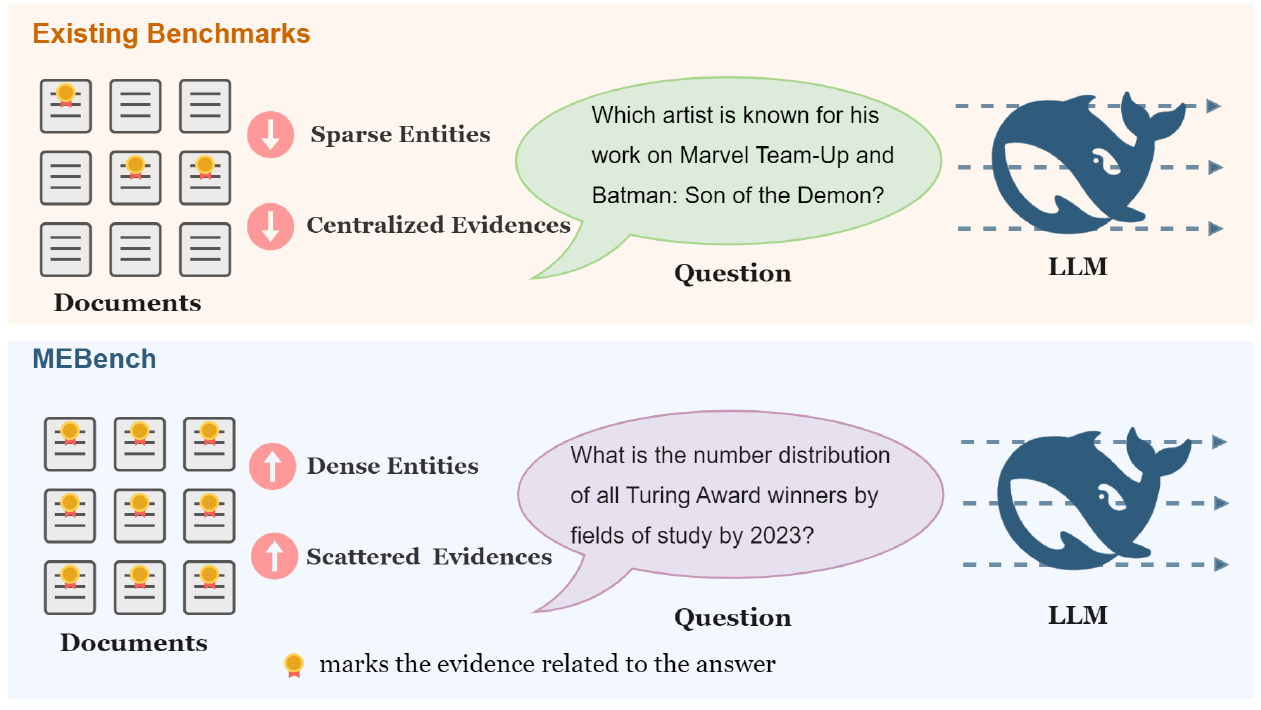
\includegraphics[width=0.6\textwidth]{rysunki/benchmarks_vs_mebench.png}
        \captionof{figure}{ Porównanie istniejących benchmarków z MEBench \cite{art1_2025}}
        \label{benchmarks_vs_mebench}
    \end{center}

    Schemat (ang. \textit{pipeline}) budowania benchmarku MEBech składa się z trzech etapów. Pierwszym z nich jest zebranie niezbędnych dokumentów. Duży model językowy GPT-4 pobiera dokumenty z Wikipedii za pomocą dedykowanego API. Dotyczą one pewnego obszaru wiedzy. W następnym kroku, zwanym ekstrakcją informacji, te dane są przetwarzane za pomocą małego modelu językowego (SLM) tak, aby na ich podstawie uzyskać ustrukturyzowaną bazę danych. Ostatnim krokiem jest generowanie pytań i odpowiedzi. Pytania są tworzone za pomocą LLMa na podstawie predefiniowanego szablonu (struktury). Następnie, model przekształca je z języka naturalnego na kwerendy bazodanowe. Na podstawie wyników tych zapytań tworzone są odpowiedzi w języku naturalnym. Poprawność odpowiedzi jest gwarantowana dzięki programowej weryfikacji, a nie na podstawie wiedzy modelu. Tak przygotowane pytania i odpowiedzi zapisywane są do oddzielnej bazy danych, którą wykorzystuje się do testów modeli. Na poniższym rysunku \ref{mebench_pipeline}, autorzy omawianego artykułu szczegółowo zaprezentowali przebieg tworzenia frameworka MEBench na przykładzie danych dotyczących członków ACM (ACM Fellows).
    
    \begin{center}
        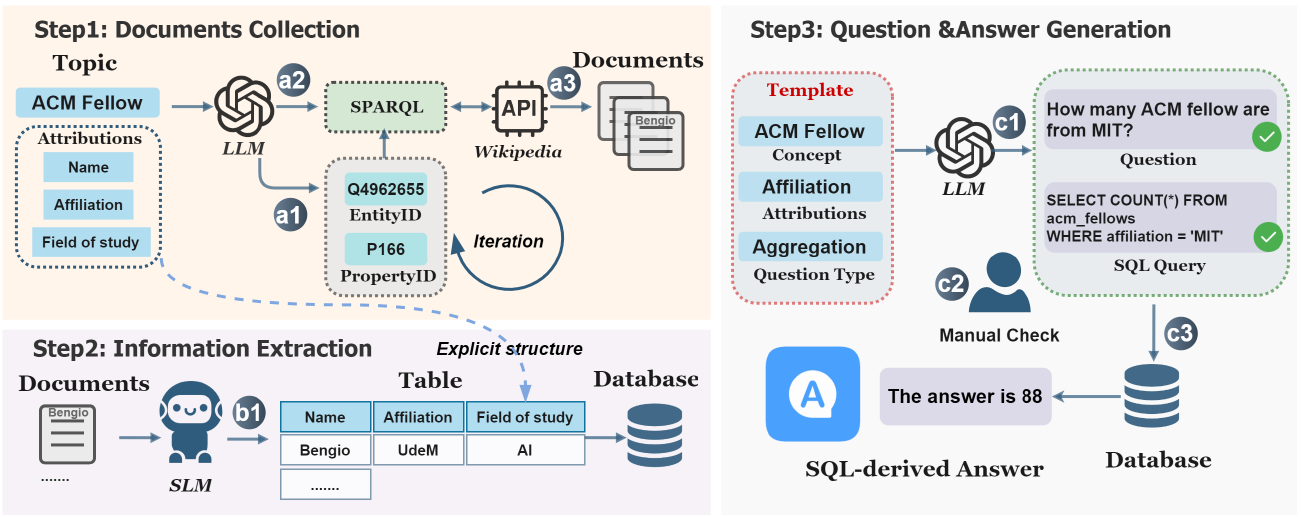
\includegraphics[width=0.85\textwidth]{rysunki/mebench_pipeline.png}
        \captionof{figure}{ Schemat tworzenia benchmarku MEBench \cite{art1_2025}}
        \label{mebench_pipeline}
    \end{center}

    Benchmark składa się 4780 pytań, które podzielone są na 3406 pytań treningowych i 1374 pytań testujących. Zebrane dane dzielone są na trzy grupy bazując na ich złożoności — mało, średnio i bardzo złożone. Do badań użyto otwartoźródłowego modelu Llama-3-Instruct (oznaczonego z dopiskiem FT) oraz zamknięte (komercyjne) modele: GPT-3.5-turbo i GPT-4. Warto podkreślić, że pytania treningowe są  wykorzystywane tylko do dostrojenia otwartoźródłowego LLMa. Wszystkie modele poddano ewaluacji w dwóch wariantach: bazowym, opierającym się wyłącznie na wiedzy parametrycznej oraz rozszerzonym o system RAG. Poniższy rysunek \ref{mebench_accuracy} przedstawia porównanie skuteczności odpowiedzi modeli, mierzonej jako dokładność (ang. \textit{accuracy}).

    \begin{center}
        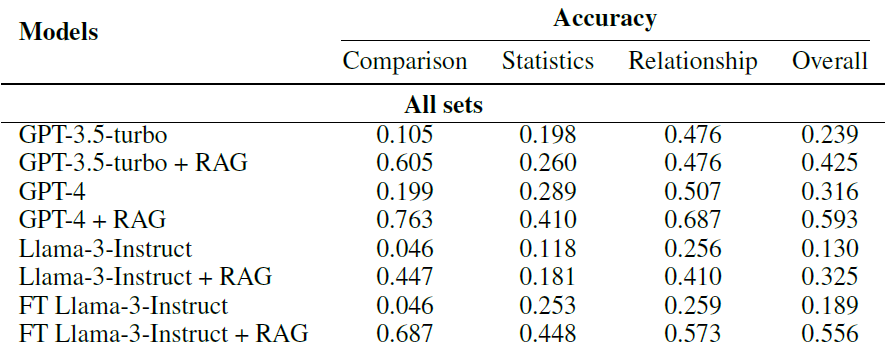
\includegraphics[width=0.75\textwidth]{rysunki/mebench_accuracy.png}
        \captionof{figure}{ Skuteczność modeli językowych w benchmarku MEBench z podziałem na kategorie pytań testowych \cite{art1_2025}}
        \label{mebench_accuracy}
    \end{center}

    Na podstawie wyników można wywnioskować, iż system GPT-4 + RAG osiągnął najwyższą dokładność wynoszącą 59,3\%. W szczególności, najlepiej poradził sobie w pytaniach porównawczych i relacyjnych. Na drugim miejscu uplasował się model FT Llama-3-Instruct z wynikiem 55,6\%. Na tle innych, najbardziej wyróżnił się w kontekście pytań statystycznych. Pytania te w ogólności stanowiły największe wyzwanie dla badanych systemów, co skutkowało najmniej satysfakcjonującymi wynikami. MEBench skutecznie wskazuje niedociągnięcia obecnych modeli LLM, ale także stanowi motywację do rozwoju solidnych architektur systemów QA, które precyzyjnie uwzględniają specyfikę zróżnicowanych zestawów danych.


    \section{Benchmark RGB}
    Drugim omawianym artykułem jest \enquote{Benchmarking Large Language Models in Retrieval-Augmented Generation} \cite{art2_unstructured2024}. Autorzy tej pracy przeanalizowali skuteczność różnych dużych modeli językowych działających w ramach systemu RAG, gdzie zewnętrznym źródłem wiedzy były dane nieustrukturyzowane. Testy przeprowadzono odpytując LLMy łącznie tysiącem pytań z czterech podstawowych kategorii: odporność na szum, odmowa odpowiedzi, integracja informacji oraz odporność na błędne fakty. W poniższej tabeli \ref{rgb_kategorie_pytan} zdefiniowano każdą z nich.

    \begin{table}[h]
        \centering
        \caption{ Definicja czterech kategorii pytań tworzących benchmark RGB }
        \begin{tabularx}{\textwidth}{|p{4.5cm}|X|}
        \hline
        \textbf{Kategoria pytań} & \textbf{Definicja} \\
        \hline
        Odporność na szum (ang. \textit{noise robustness}) & Umożliwia sprawdzenie czy LLM potrafi wydobywać użyteczne informacje z zaszumionych dokumentów.  \\ \hline
        
        Odmowa odpowiedzi (ang. \textit{negative rejection}) & Pozwala zbadać czy LLM odmówi odpowiedzi na pytanie, kiedy nie ma wystarczającej ilości danych na konkretny temat w żadnym dokumencie.  \\ \hline
        
        Integracja informacji (ang. \textit{information integration}) & Służy do sprawdzenia czy LLM jest w stanie odpowiedzieć na złożone pytania wymuszające zebranie i połączenie ze sobą informacji z wielu dokumentów. \\ \hline

        Odporność na błędne fakty (ang. \textit{counterfactual robustness}) & Umożliwia sprawdzenie czy LLM potrafi wskazać błędne fakty w dokumentach bazując na swojej wiedzy parametrycznej. W wiadomości systemowej modelu powinno być wspomniane, że dokumenty mogą zawierać błędy. \\ \hline
        \end{tabularx}
        \label{rgb_kategorie_pytan}
    \end{table}

    \noindent W celu przeprowadzenia testów, autorzy utworzyli test wydajnościowy Retrieval-Augmented Generation Benchmark (RGB). Jest to najnowszy framework do ewaluacji systemu RAG dla języka angielskiego i chińskiego. RGB jest podzielony na cztery oddzielne zestawy testów. Każdy z nich odpowiada wyżej wymienionym kategoriom pytań, które są zadawane sześciu ówcześnie najnowocześniejszym modelom językowym: GPT-3.5-turbo, ChatGLM-6B, ChatGLM2-6B, Vicuna-7b-v1.3, Qwen-7B-Chat oraz BELLE-7B-2M.

    W celu wygenerowania pytań i odpowiedzi do przypadków testowych w benchmarku, bazując na najaktualniejszych źródłach danych z internetu, stosuje się ChatGPT. Na podstawie zewnętrznych dokumentów tworzy on krótkie opisy najważniejszych wydarzeń, pytania i odpowiedzi. Tak utworzone treści są ręcznie filtrowane przez twórców. Pytania są dzielone na opisane wcześniej cztery różne grupy. Dla każdego zapytania zostaje użyte API Google do zaciągnięcia dziesięciu istotnych stron internetowych. Te zewnętrzne dokumenty są następnie dzielone na pozytywne i negatywne w zależności od tego czy zawierają odpowiedź czy nie. Dopiero ten zaciągnięty zbiór dokumentów służy jako zewnętrzna wiedza modelu w systemie RAG.

    Ewaluację modeli językowych przeprowadzono oddzielnie dla każdego z czterech zestawów testowych. Poniższy rysunek \ref{rgb_4_kategorie_pytan} prezentuje przykład pytań i odpowiedzi z każdej kategorii.

    \begin{center}
        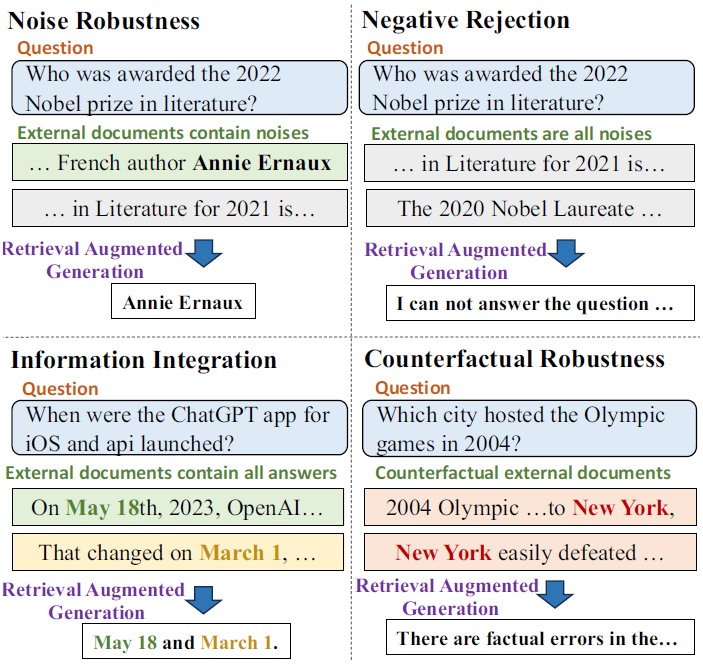
\includegraphics[width=0.6\textwidth]{rysunki/rgb_4_kategorie_pytan.png}
        \captionof{figure}{ Przykład pytań i odpowiedzi dla czterech zestawów testowych służących do ewaluacji systemów RAG w ramach benchmarku RGB \cite{art2_unstructured2024}}
        \label{rgb_4_kategorie_pytan}
    \end{center}

    \noindent W wynikach pierwszego testu zauważono, że LLMy wykazały się dużą zdolnością odfiltrowania istotnych informacji z zaszumionych danych, czyniąc RAG obiecującą techniką rozszerzającą zdolności modeli językowych. Natomiast, gdy stopień zaszumienia przekroczył 80\%, dokładność odpowiedzi modeli znacząco spadła, o około 15\% dla każdego z nich. W tym podejściu ChatGPT osiągnął najlepsze wyniki. W drugim teście dostrzeżono, że odmowa odpowiedzi modeli stanowi największe wyzwanie. Najwyższym wskaźnikiem odmowy odznaczył się model GPT ze skutecznością 45\%. Odnośnie pytań z trzeciej kategorii, modele poradziły sobie nieco lepiej. Najwyższą skutecznością integracji informacji wykazał się model Qwen na poziomie 67\%. Jak łatwo zauważyć, pytania z tej dziedziny także stanowią duże wyzwanie dla modeli językowych. Dla pytań z ostatniej grupy testowej, ChatGPT poradził sobie najlepiej. Wykazał się on znajomością faktów bazując tylko na wewnętrznej parametrycznej wiedzy na poziomie 91\%. Natomiast, przy dołączonych zewnętrznych dokumentach zawierających przeciwstawne fakty, wykazał się on już skutecznością na poziomie 17\%, co i tak okazało się być najlepszym wynikiem. Rezultaty eksperymentów dla benchmarku RGB wskazują, że LLMy mają ograniczenia dla każdej z czterech kategorii pytań. Dowodzi to, że aby zapewnić dokładne i wiarygodne odpowiedzi dużych modeli językowych kluczowe jest zachowanie ostrożności i staranne projektowanie systemów RAG.
    

    \section{Benchmark NL-to-SQL} 

    W artykule \enquote{Benchmarking Large Language Models for NL-to-SQL: A Comprehensive Evaluation of Accuracy, Cost and Throughput} \cite{art3_structured2024} autorzy skupili się na rozwoju benchmarku pozwalającego na ewaluację dużych modeli językowych w kontekście systemu RAG, gdzie zewnętrznym źródłem ustrukturyzowanych danych jest baza danych SQL. Sprawdzono jak modele radzą sobie z zamianą języka naturalnego na kwerendy bazodanowe (NL-to-SQL). Przetestowano LLMy na różnych platformach za pomocą łącznie 360 pytań selektywnie wybranych ze zbioru danych BIRD \cite{bird2018}. Były to kwerendy o następujących poziomach zaawansowania: łatwe, umiarkowane i trudne \cite{3_levels_of_questions_difficulty2023}. Poziom trudności zdefiniowano na podstawie liczby komponentów SQL, selekcji oraz warunków, tak aby zapytania zawierające większą liczbę słów kluczowych SQL były uznawane za trudniejsze. Na sześciu różnych platformach hostingowych przebadano łącznie 30 modeli (niektóre z nich się powtarzały). Poniżej w tabeli \ref{nltosql_modele} wypisano wszystkie z nich.    

    \begin{table}[h]
        \centering
        \caption{ Platformy i przypisane do nich LLMy badane w ramach benchmarku NL-to-SQL \cite{art3_structured2024}}
        \begin{tabularx}{\textwidth}{|p{3cm}|X|}
        \hline
        \textbf{Platforma} & \textbf{Modele LLM} \\
        \hline
        Anyscale & Llama3-70B, Llama2-70B, Mistral 7B (Version 1), Mixtral8x7B, CodeLlama-70B  \\ \hline
        
        Amazon Bedrock & Llama3-70B, Llama2-70B, Mistral-7B (Version 2), Mixtral8x7B, Claude3-Sonnet, Claude3-Haiku  \\ \hline
        
        OpenAI  & GPT3.5 Turbo, GPT4 Turbo, GPT4 omni, GPT4o mini  \\ \hline

        Anthropic & Claude3-Opus, Claude3-Sonnet, Claude3-Haiku, Claude3.5-Sonnet  \\ \hline

        Google & Gemini 1.0 Pro  \\ \hline

        Własny hosting & DBRX Instruct, Llama3-70B, CodeLlma-70B, CodeLlma-34B, Mistral-7B (Version 1), Mistral-7B (Version 2), Mixtral8x7B, Sql Coder 7B2, Sql Coder 70B Alpha, WizardCoder-33B  \\ \hline
        \end{tabularx}
        \label{nltosql_modele}
    \end{table}

    Takie podejście pozwoliło autorom dokładnie porównać modele pod kątem wydajności, przepustowości (szybkości odpowiedzi) oraz kosztu odpowiedzi w różnych środowiskach hostingowych. Warto podkreślić, że przepustowość oblicza się ze wzoru \ref{wzór_przepustowość_odpowiedzi_llm}, gdzie $N_{output}$ oznacza całkowitą liczbę tokenów wygenerowanych w odpowiedzi, a $t_{response}$ oznacza czas generowania tej odpowiedzi przez LLM.

    \begin{equation}
        \begin{aligned}
            T = \frac{N_{output}}{t_{response}}
        \end{aligned}
        \label{wzór_przepustowość_odpowiedzi_llm}
    \end{equation}

    \noindent Koszt odpowiedzi policzono ze znajdującego się poniżej wzoru \ref{wzór_koszt_odpowiedzi_llm}, gdzie \enquote{mil} jest skrótem od \enquote{milionów}, a \enquote{tok} jest skrótem od \enquote{tokenów}.

    \begin{equation}
        \begin{aligned}
            C = {} & \text{Koszt promptu za mil tok} \times \text{Liczba tok wejściowych} \\
            & + \text{Koszt odpowiedzi za mil tok} \times \text{Liczba tok wyjściowych}
        \end{aligned}
        \label{wzór_koszt_odpowiedzi_llm}
    \end{equation}

    \noindent Na rysunku \ref{nltosql_dokladnosc_odpowiedzi} zaprezentowano zestawienie wszystkich przetestowanych modeli uwzględniając dokładność odpowiedzi oznaczoną na osi poziomej jako EX (Execution Accuracy). Jak widać, najlepiej poradziły sobie modele GPT-4o i Claude-3.5 Sonnet z dokładnościami odpowiednio: 41.44\% i 40.94\%. Natomiast, najgorzej poradził sobie model Llama2-70B hostowany na platformie Amazon Bedrock (2.11\%). Modele hostowane na tym środowisku wykazują się średnio najmniejszą trafnością odpowiedzi. Łatwo zauważyć, iż całokształt nie jest satysfakcjonujący. Modele LLM potrafiły odpowiedzieć średnio na co trzecie pytanie bazodanowe. W zastosowaniach praktycznych zniechęcałoby to użytkownika do konwersacji z chatbotem. Bardziej odpowiednim rozwiązaniem w tym przypadku byłoby bezpośrednie odpytywanie bazy danych.

    \begin{center}
        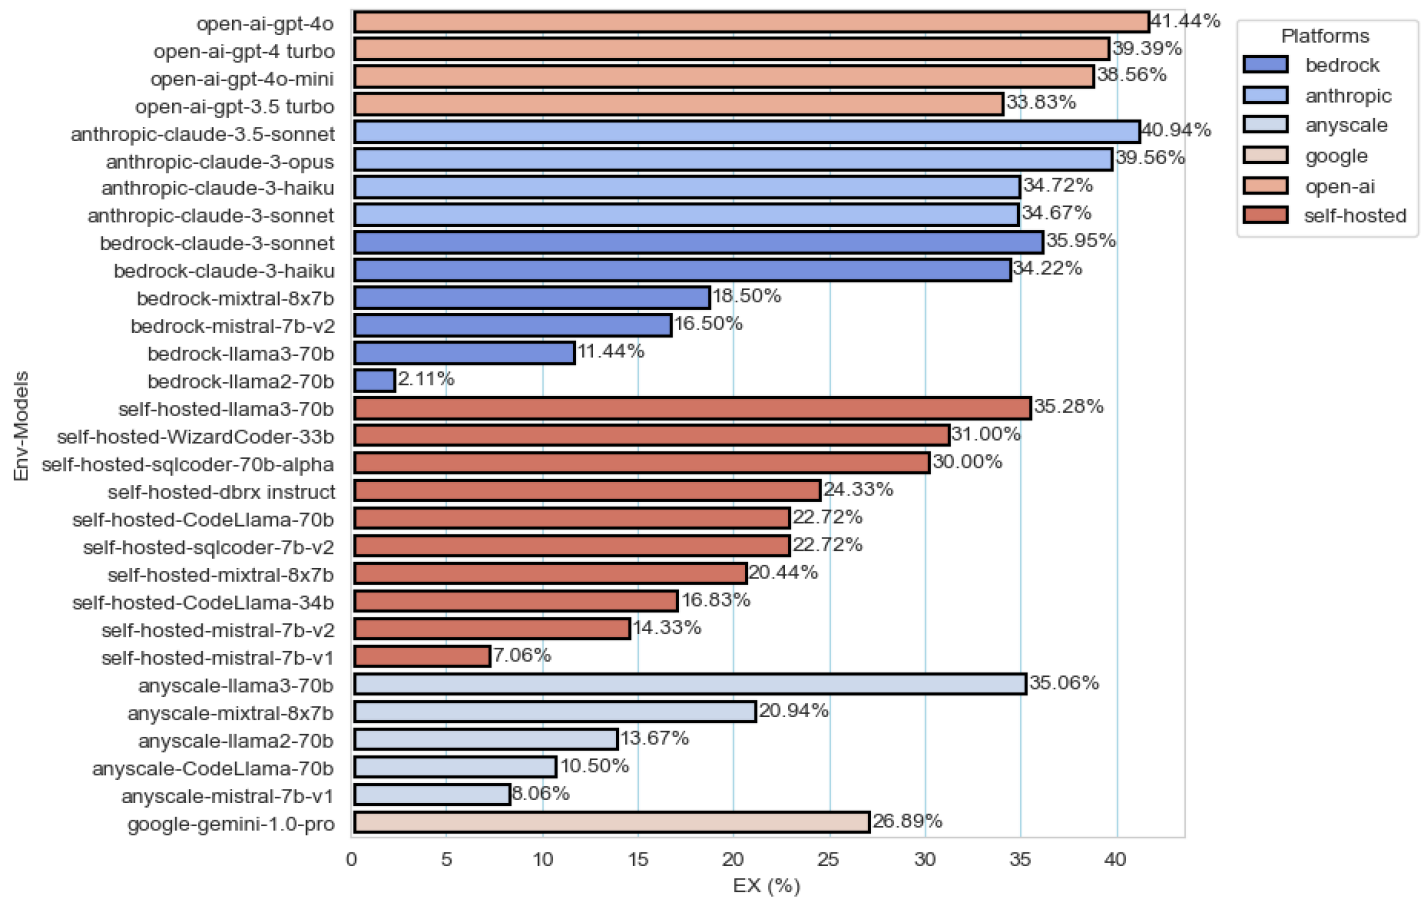
\includegraphics[width=0.8\textwidth]{rysunki/nltosql_dokladnosc_odpowiedzi.png}
        \captionof{figure}{ Dokładności modeli w zależności od platform hostujących w ramach benchmarku NL-to-SQL \cite{art3_structured2024}}
        \label{nltosql_dokladnosc_odpowiedzi}
    \end{center}

    \noindent Na następnym rysunku \ref{nltosql_koszt_odpowiedzi} przedstawiono średni koszt generowania odpowiedzi przez zewnętrznie hostowane modele w zależności od poziomu zaawansowania pytań. Model Claude3-Opus na platformie Anthropic okazał sie być najdroższym ze wszystkich modeli. Średni koszt wygenerowania wszystkich odpowiedzi w ramach testów wyniósł aż \$15.76. Jedynym darmowym modelem był Gemini 1.0 Pro, którego użycie skutkowało brakiem opłat za wygenerowanie wszystkich odpowiedzi. Z przytoczonych danych można wywnioskować, że wyższa cena modelu nie zawsze oznacza proporcjonalnie lepszą jakość.

    \begin{center}
        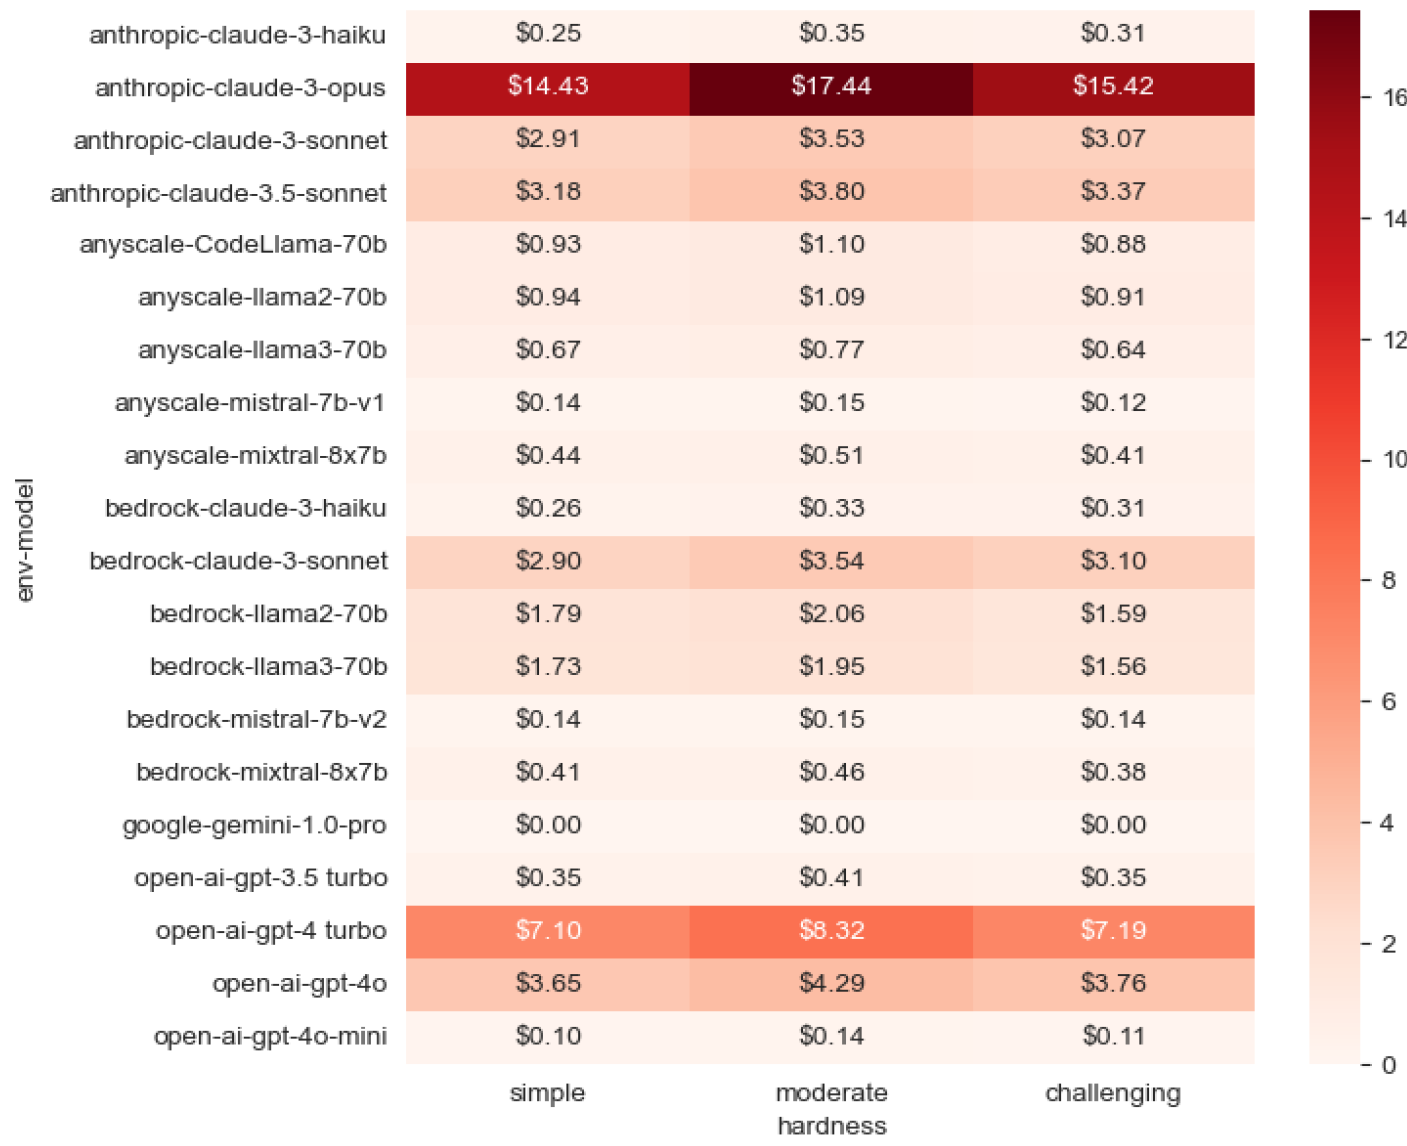
\includegraphics[width=0.7\textwidth]{rysunki/nltosql_koszt_odpowiedzi.png}
        \captionof{figure}{ Średnie koszty (w dolarze \$) generowania odpowiedzi dla zewnętrznie hostowanych modeli w zależności od stopnia zaawansowania pytań w ramach benchmarku NL-to-SQL \cite{art3_structured2024}}
        \label{nltosql_koszt_odpowiedzi}
    \end{center}

    \noindent Trzecim wartym uwagi wykresem jest ten wizualizujący średnią przepustowość modeli na wszystkich platformach w zależności od poziomu zaawansowania pytań \ref{nltosql_przepustowosc_modeli}. W tej kategorii najlepiej poradził sobie model Mistral-7B (Version 2) hostowany na platformie Amazon Bedrock. Jego średnia przepustowość wyniosła 87.11 t/s. Dla porównania, najmniejszą przepustowością wykazał się DBRX Instruct i wyniosła ona tylko 14.81 t/s.

    \begin{center}
        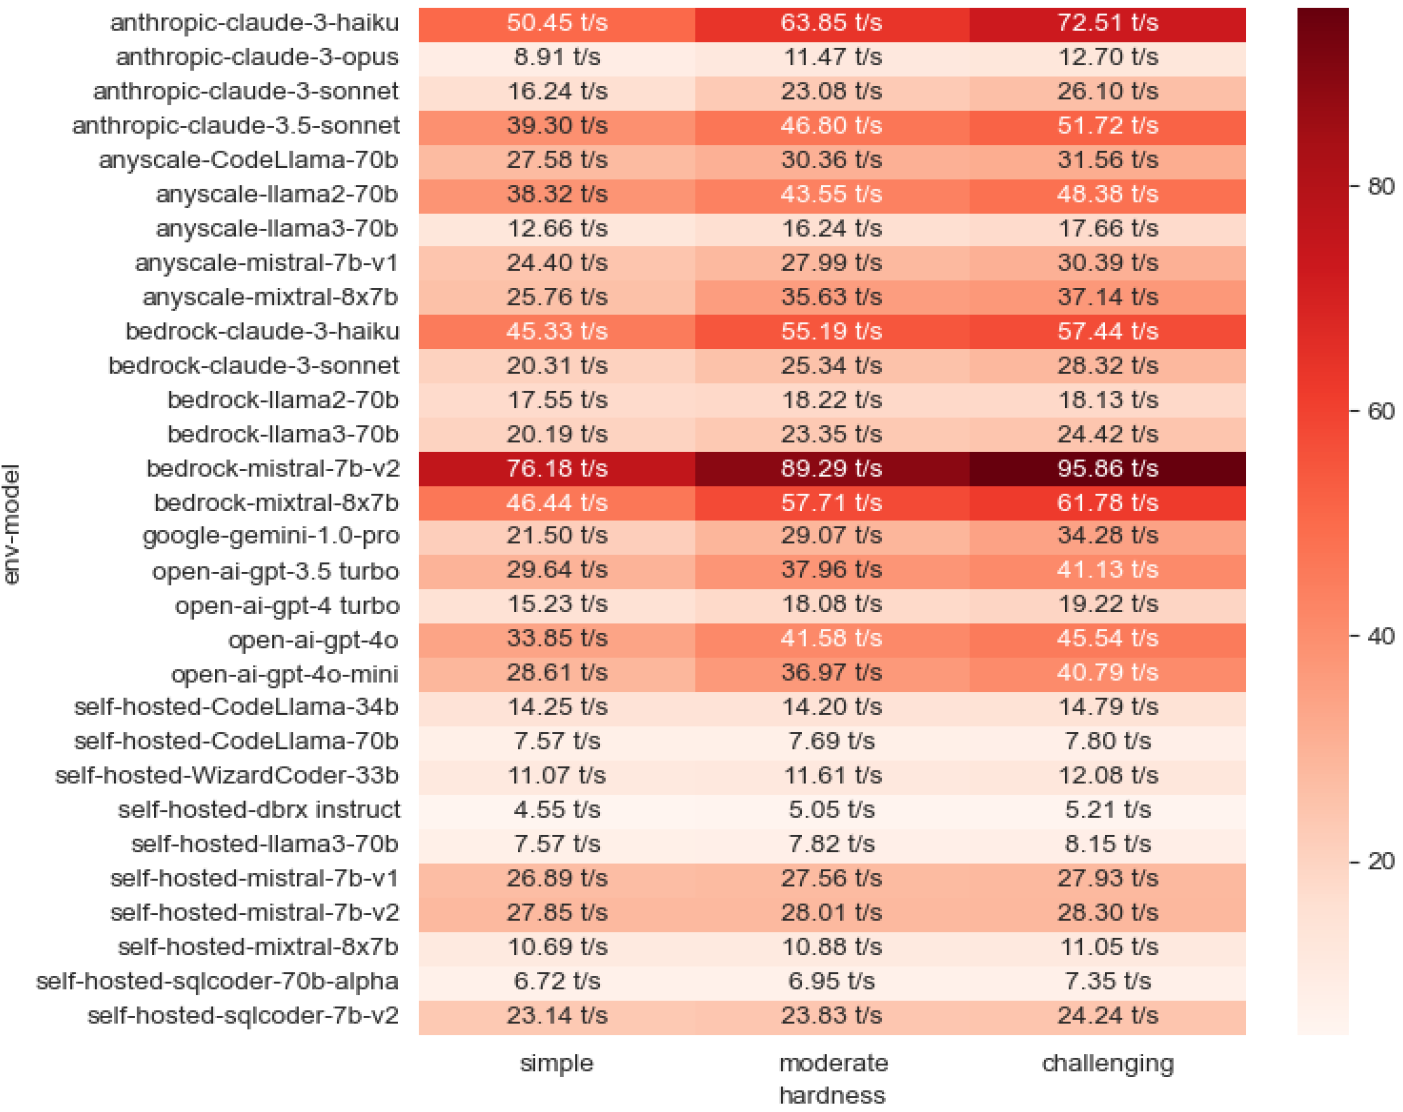
\includegraphics[width=0.7\textwidth]{rysunki/nltosql_przepustowosc_modeli.png}
        \captionof{figure}{ Średnie przepustowości (w tokenach na sekundę t/s) podczas generowania odpowiedzi dla wszystkich modeli w zależności od stopnia zaawansowania pytań w ramach benchmarku NL-to-SQL \cite{art3_structured2024}}
        \label{nltosql_przepustowosc_modeli}
    \end{center}

    \noindent Kompleksowe wyniki z artykułu wykazują, że wraz ze wzrostem trudności pytania, modelowi trudniej jest na nie trafnie odpowiedzieć. Co ciekawe, przepustowość rośnie proporcjonalnie do stopnia zaawansowania kwerendy. Najbardziej kosztowne okazało się generowanie odpowiedzi na średniozaawansowane pytania. Dalsze prace nad modelami LLM w zadaniach NL-to-SQL powinny koncentrować się na wdrażaniu technik few-shot learning, RAG i fine-tuningu oraz na optymalizacji wydajności i kosztów rozwiązań w ramach własnego hostingu.
\cleardoublepage

\chapter{Badanie dużych modeli językowych w systemach RAG za pomocą autorskiego rozwiązania}

W tym rozdziale skupiono się na części praktycznej niniejszej pracy dyplomowej. Autor zaprezentował autorskie systemy RAG służące do testów dominujących dużych modeli językowych w zakresie odpowiadania na pytania dotyczące zewnętrznych nieustrukturyzowanych i ustrukturyzowanych źródeł danych. Badanie odbyło się 29 marca 2026 roku.


    \section{Cel badania}
    Celem badania było przetestowanie i porównanie pięciu popularnych i najnowszych dużych modeli językowych w zakresie trafności, kosztu, czasu i przepustowości tokenów generowanych odpowiedzi w oparciu o zewnętrzne źródła wiedzy. Były to następujące modele pięciu różnych liderów w zakresie GenAI: gpt-5-mini, deepseek-v3.2-exp, gemini-3-flash-preview, claude-haiku-4.5 i grok-4.1-fast. Do testów wykorzystano łącznie cztery ustrukturyzowane i nieustrukturyzowane zestawy danych. Wobec każdego z nich sformułowano 8 pytań z czterech kategorii. Każde pytanie zadano jednokrotnie dla każdej konfiguracji. Do stworzenia autorskich systemów RAG posłużyła platforma n8n \cite{n8n} stosowana do automatyzacji zadań i procesów. Po wykonanych testach, wykonano analizę wyników i wybrał optymalną konfigurację systemu.


    \section{Przygotowanie danych}
    Jako danych nieustrukturyzowanych użyto jedenastostronnicowego pliku PDF oraz pliku tekstowego. Oba odnosiły się do tego samego artykułu internetowego pt.: \enquote{Czym są duże modele językowe?} \cite{oracle_czym_sa_llm}. Pierwszy plik został stworzony poprzez bezpośrednie przekonwertowanie strony internetowej na PDF. Drugi plik powstał poprzez scraping treści z tej samej strony do formatu markdown, co później zostało zapisane do formatu .txt. Udało się to osiągnąć za pomocą platformy Firecrawl \cite{firecrawl}. Należy zaznaczyć, iż oba pliki w jednym miejscu zostały zmodyfikowane. Jedno z dwóch wystąpień roku \enquote{2017} zmieniono na \enquote{2002}. Modyfikacja ta została dokonana na potrzeby badania. Docelowo zawartości obu plików poddano procesowi wektoryzacji i zaindeksowania w bazie danych Pinecone \cite{pinecone}. Na poniższym rysunku \ref{vector_store_embedding_n8n} przedstawiono autorskie oprogramowanie wykonujące ten proces.

    \begin{center}
        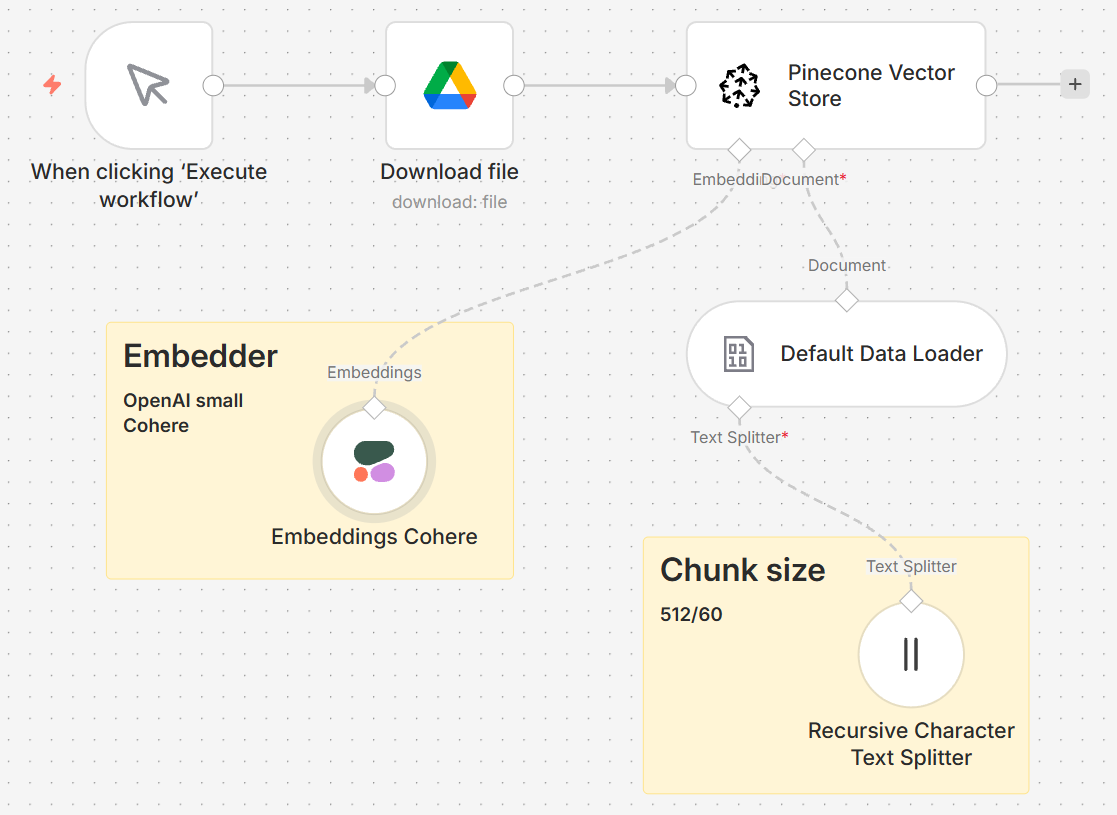
\includegraphics[width=0.5\textwidth]{rysunki/vector_store_embedding_n8n.png}
        \captionof{figure}{ Workflow w n8n służący do transformacji nieustrukturyzowanych danych w embeddingi zapisane do wektorowej bazy danych Pinecone \cite{n8n} }
        \label{vector_store_embedding_n8n}
    \end{center}

    \noindent W ramach przedstawionego workflow zastosowano segmentację tekstu (chunking) na fragmenty o długości 512 tokenów z marginesem części wspólnej (overlapping) wynoszącym 60 tokenów. Dla każdego z plików proces ten uruchomiono dwukrotnie, wykorzystując dwa różne modele osadzające: text-embedding-3-small od OpenAI (o wymiarowości 1536) oraz Embed-Multilingual-v3.0 od Cohere (o wymiarowości 1024). Dzięki temu, na platformie Pinecone przechowano cztery różne wektorowe bazy danych: pdf-openai, pdf-cohere, scraped-openai i scraped-cohere. Doskonale posłużyły one jako zewnętrzne źródła nieustrukturyzowanej wiedzy podczas testowania modeli w ramach systemów RAG.
    
    Jako źródło danych ustrukturyzowanych użyto bazę danych SQL i plik CSV. Oba zasoby zawierały takie same rekordy i zostały stworzone na podstawie ogólnodostępnego pliku products100.csv z repozytorium \enquote{sample-csv-files} na platformie GitHub \cite{products100_github}. Posiadał on 100 rekordów i następujące kolumny (atrybuty): Index, Name, Description, Brand, Category, Price, Currency, Stock, EAN, Color, Size, Availability, Internal\_ID. Do przechowania bazy SQL wykorzystano platformę Supabase \cite{supabase}, która działa w oparciu o system Postgres. Plik CSV znajdował się bezpośrednio na platformie n8n. Warto podkreślić, że żaden z plików nie został zmodyfikowany.


    \section{Przygotowanie pytań}
    Do testowania modeli językowych w dedykowanym systemie RAG autor utworzył dwa zestawy pytań \ref{pytania_nieustrukturyzowane} i \ref{pytania_ustrukturyzowane}. Pierwszy dotyczył danych nieustrukturyzowanych, a drugi danych ustrukturyzowanych. Podczas kreowania pytań zainspirowano się odpowiednimi artykułami naukowymi omawianymi w poprzednim rozdziale \cite{art2_unstructured2024} i \cite{art3_structured2024}.
        
    \begin{table}[h]
        \centering
        \caption{ Pytania do nieustrukturyzowanych źródeł danych }        
        \begin{tabularx}{\textwidth}{|l|X|}
        \hline
        \textbf{Kategoria} & \textbf{Pytanie} \\ \hline
        
        \multirow{4}{*}{Integracja informacji} & Jaki produkt firmy OpenAI jest powszechnie uważany za pierwszy współczesny model LLM i ile miał on parametrów? \\ \cline{2-2} 
         & Który model stworzony przez OpenAI uznaje się za pionierski w kategorii współczesnych LLM i jaka była skala jego parametrów? \\ \hline
        
        \multirow{4}{*}{Odporność na szum} & Jak automatyzacja z użyciem LLM wpływa na produktywność w komunikacji z klientami? \\ \cline{2-2} 
         & W jaki sposób wykorzystanie modeli językowych do automatyzacji przekłada się na efektywność obsługi klienta? \\ \hline
        
        \multirow{5}{*}{Odporność na błędne fakty} & W którym roku naukowcy z Google opublikowali artykuł wprowadzający architekturę Transformer? \\ \cline{2-2} 
         & Kiedy światło dzienne ujrzał przełomowy artykuł Google prezentujący nową architekturę, będącą fundamentem obecnego przełomu w generatywnej sztucznej inteligencji? \\ \hline
        
        \multirow{3}{*}{Odmowa odpowiedzi} & Kto jest szefem firmy OpenAI? \\ \cline{2-2} 
         & Na podstawie załączonego dokumentu wskaż, kto pełni funkcję dyrektora generalnego (CEO) firmy OpenAI. \\ \hline
        
        \end{tabularx}
        \label{pytania_nieustrukturyzowane}
    \end{table}

    Pierwszy zestaw pytań składał się z czterech kategorii: integracja informacji, odporność na szum, odporność na błędne fakty i odmowa odpowiedzi. Każda zawierała po dwa pytania dotyczące tej samej kwestii, jednak sformułowane na dwa różne sposoby. Łącznie było 8 pytań. Zgodnie z zewnętrznym źródłem wiedzy, odpowiedzi na pytania z każdej kategorii powinny odpowiednio przypominać poniższe, stanowiące punkt odniesienia:
    
    \begin{itemize}
        \item \enquote{\textit{Pierwszym współczesnym modelem LLM od firmy OpenAI był GPT-1 i posiadał on nieco ponad 100 milionów parametrów.}},
        
        \item \enquote{\textit{LLM znacząco podnosi produktywność w komunikacji z klientami: skracają czas oczekiwania i odciążają personel przez całodobowe, wielojęzyczne czatboty oraz automatyzację zadań follow‑up.  Istotnie wpływa na wzrost poziomu usług o 150\% i spadek kosztów o 30\%.}},
        
        \item \enquote{\textit{Artykuł Google wprowadzający architekturę Transormer ukazał się w 2017 roku. W jednym fragmencie dokumentu występuje błąd — podano tam 2002, a prawidłowy rok to 2017.}},
        
        \item \enquote{\textit{Niestety, nie umiem odpowiedzieć na to pytanie na podstawie dostępnego artykułu.}}.
    \end{itemize}

    \noindent Warto nadmienić, że w ramach niniejszego projektu, trzecia kategoria posłużyła sprawdzeniu czy LLM jest w stanie odpowiedzieć na złożone pytania wymuszające zebranie i połączenie ze sobą informacji z wielu sekcji (akapitów) pojedynczego dokumentu, a nie z wielu dokumentów. 

    \begin{table}[h]
        \centering
        \caption{ Pytania do ustrukturyzowanych źródeł danych }        
        \begin{tabularx}{\textwidth}{|l|X|}
        \hline
        \textbf{Kategoria} & \textbf{Pytanie} \\ \hline
        
        \multirow{2}{*}{Łatwe} & Ile produktów jest w bazie? \\ \cline{2-2} 
         & Ile kosztuje rower? \\ \hline
        
        \multirow{2}{*}{Umiarkowane} & Które produkty kosztują więcej niż 920 USD? \\ \cline{2-2} 
         & Wypisz produkty, których 'Internal\_ID' wynosi 3. \\ \hline
        
        \multirow{3}{*}{Trudne} & Ile łącznie kosztują produkty: Smart Lamp, Eco Radio i Fast Keyboard? \\ \cline{2-2} 
         & Jaka jest łączna wartość magazynowa (Price × Stock) produktów dostępnych jako 'out\_of\_stock'? \\ \hline

         \multirow{3}{*}{Odmowa odpowiedzi} & Jaki kolor ma krzesło? \\ \cline{2-2} 
         & Na podstawie tabeli, wskaż na który produkt czas oczekiwania jest najdłuższy. \\ \hline
        
        \end{tabularx}
        \label{pytania_ustrukturyzowane}
    \end{table}

    Drugi zestaw pytań także składał się z czterech kategorii: łatwe, umiarkowane, trudne i odmowa odpowiedzi. Każda zawierała po dwa różne pytania. Łącznie było 8 zapytań. Zgodnie z zewnętrznym źródłem wiedzy, odpowiedzi na wszystkie osiem pytań powinny w odpowiedni sposób nawiązywać do poniższych przykładów, stanowiących punkt odniesienia:

    \begin{itemize}
        \item \enquote{\textit{W bazie jest 100 produktów.}},
        
        \item \enquote{\textit{Rower kosztuje 234 USD.}},
        
        \item \enquote{\textit{Jest 6 produktów kosztujących więcej niż 920 USD: Ultra Speakerphone Oven Go Smart, Fast Keyboard, Clock Brush, Eco Iron Monitor Air, Fast Fan i Rechargeable Projector.}},
        
        \item \enquote{\textit{Znaleziono 2 produkty o Internal\_ID równym 3: Smart Webcam Projector Lock i Smart Lamp}},

        \item \enquote{\textit{Łączny koszt produktów Smart Lamp, Eco Radio i Fast Keyboard wynosi 1523 USD.}},
        
        \item \enquote{\textit{Łączna wartość magazynowa produktów o statusie 'out\_of\_stock' wynosi 3 219 633 USD.}},
        
        \item \enquote{\textit{Niestety, nie umiem odpowiedzieć na to pytanie na podstawie dostępnej bazy danych.}},
        
        \item \enquote{\textit{Niestety, nie umiem odpowiedzieć na to pytanie na podstawie dostępnej bazy danych.}}.
    \end{itemize}
    
    
    \section{Przeprowadzenie testów}
    W celu przeprowadzenia testów utworzono trzy scenariusze automatyzacji testów (workflow) na platformie n8n, które przedstawiono na rysunkach \ref{mgr_unstructured_structuredSQL_n8n} i \ref{mgr_structured_csv_n8n}. Każdy z nich działał w zbliżony sposób, a jedyną różnicę stanowiły narzędzia agentów AI oraz wiadomości systemowe, które znajdują się w dołączonym do pracy pliku ZIP oraz w repozytorium plików autora na platformie GitHub \cite{moje_repozytorium}. W pierwszej kolejności należało podać prompt (zapytanie), które następnie zostało przekazane do pięciu agentów AI. Każdy z nich miał dołączony odpowiedni model, do którego dostęp zapewniało API programu OpenRouter \cite{openrouter}. Agenty AI były połączone z zewnętrznymi źródłami danych dzięki odpowiednim narzędziom, które zdefiniowano w późniejszej części bieżącej sekcji. Odpowiedzi dużych modeli językowych na zadane pytania gromadziły się następnie w węźle Merge. Tak zestawione wyniki zostały automatycznie wpisane do odpowiedniej kolumny w dedykowanym arkuszu Google. Liczbę tokenów oraz czas generowania odpowiedzi spisywano ręcznie z parametrów agentów po każdym wykonanym teście do tego samego arkusza.

    \begin{center}
        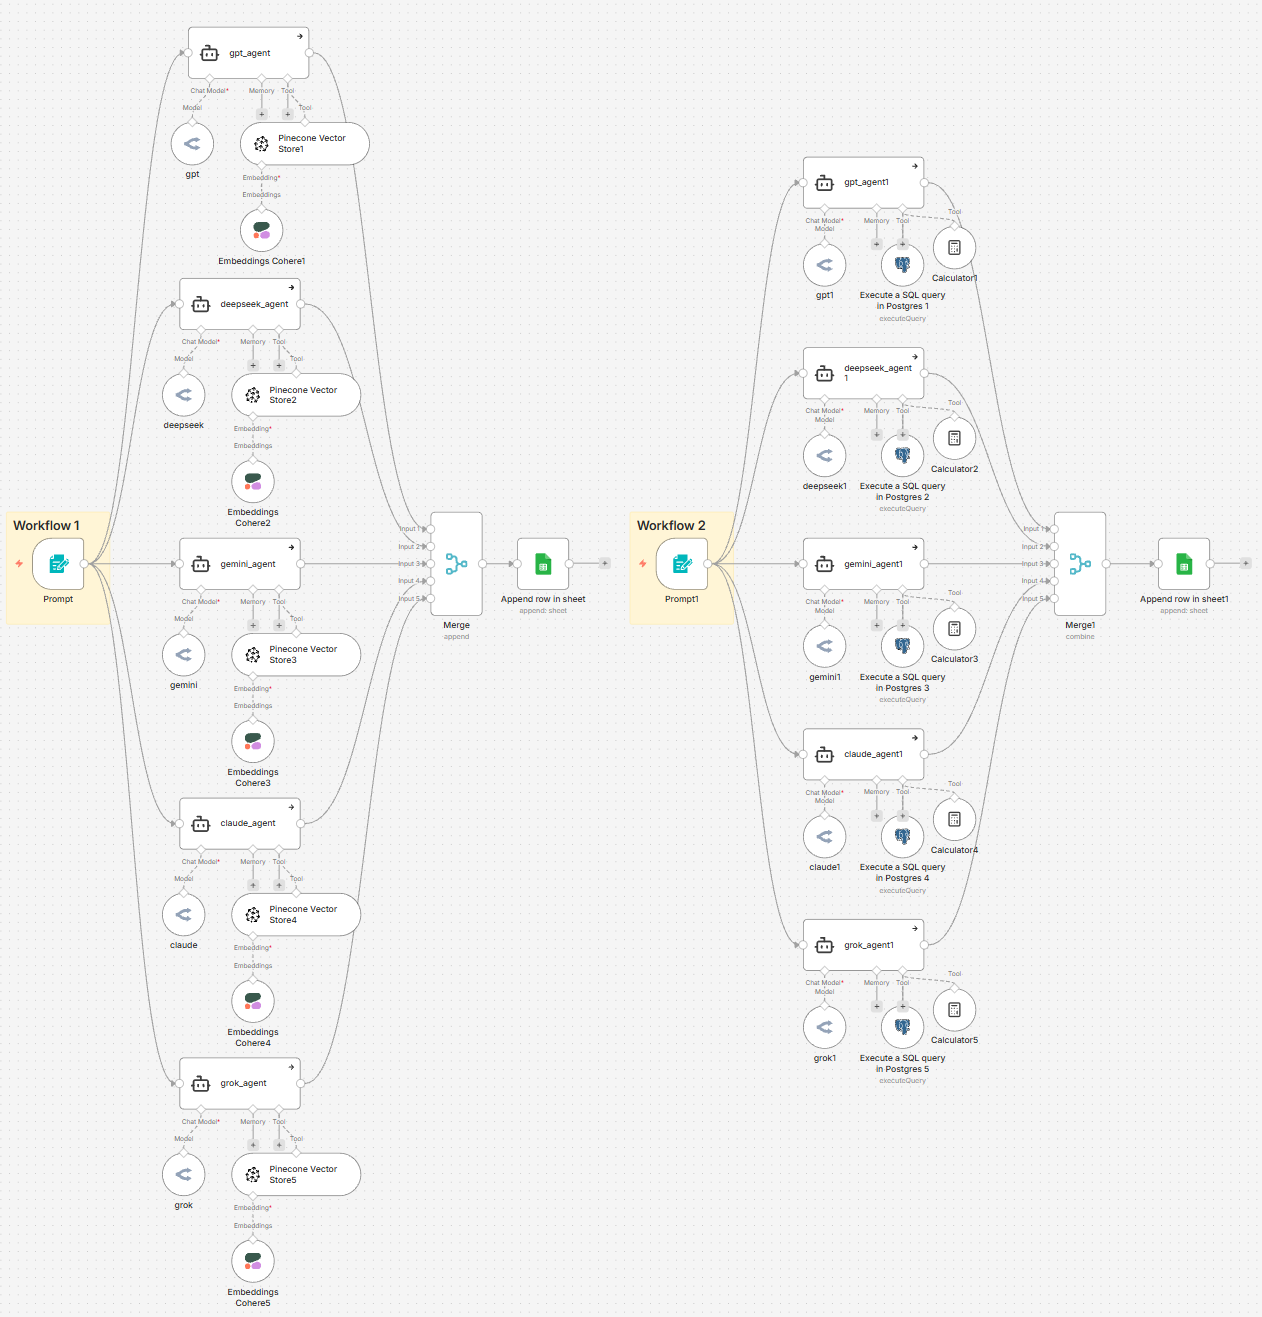
\includegraphics[width=0.8\textwidth]{rysunki/mgr_unstructured_structuredSQL_n8n.png}
        \captionof{figure}{ Dwa scenariusze automatyzacji testów systemów RAG — Workflow 1 dla dokumentu PDF i pliku tekstowego oraz Workflow 2 dla bazy danych SQL \cite{n8n}}
        \label{mgr_unstructured_structuredSQL_n8n}
    \end{center}

    W pierwszym workflow, do zewnętrznego źródła danych można było się odnieść za pomocą narzędzia dedykowanego wektorowym bazom danych Pinecone. W opisie narzędzia zawarto taką treść: \enquote{\textit{Użyj tego narzędzia, aby przeszukać bazę wektorową zawierającą treść artykułu firmy Oracle o dużych modelach językowych}}. W zależności od tego jaki embedder został użyty do utworzenia konkretnej bazy wektorowej, taki też był stosowany w danym przypadku do wydobywania niezbędnych informacji.
    
    W drugim workflow, do zewnętrznej bazy danych SQL można było się odnieść za pomocą narzędzia Postgres. Umożliwiło ono ekstrakcję danych stosując wygenerowane zapytanie w formacie SQL przez duży model językowy, aby poprawnie odpowiedzieć na zadane przez użytkownika pytanie. Dodatkowym narzędziem był kalkulator. Ułatwił on wykonywanie skomplikowanych obliczeń matematycznych, z którymi LLMy w takiej konfiguracji mają sporo trudności.

    \begin{center}
        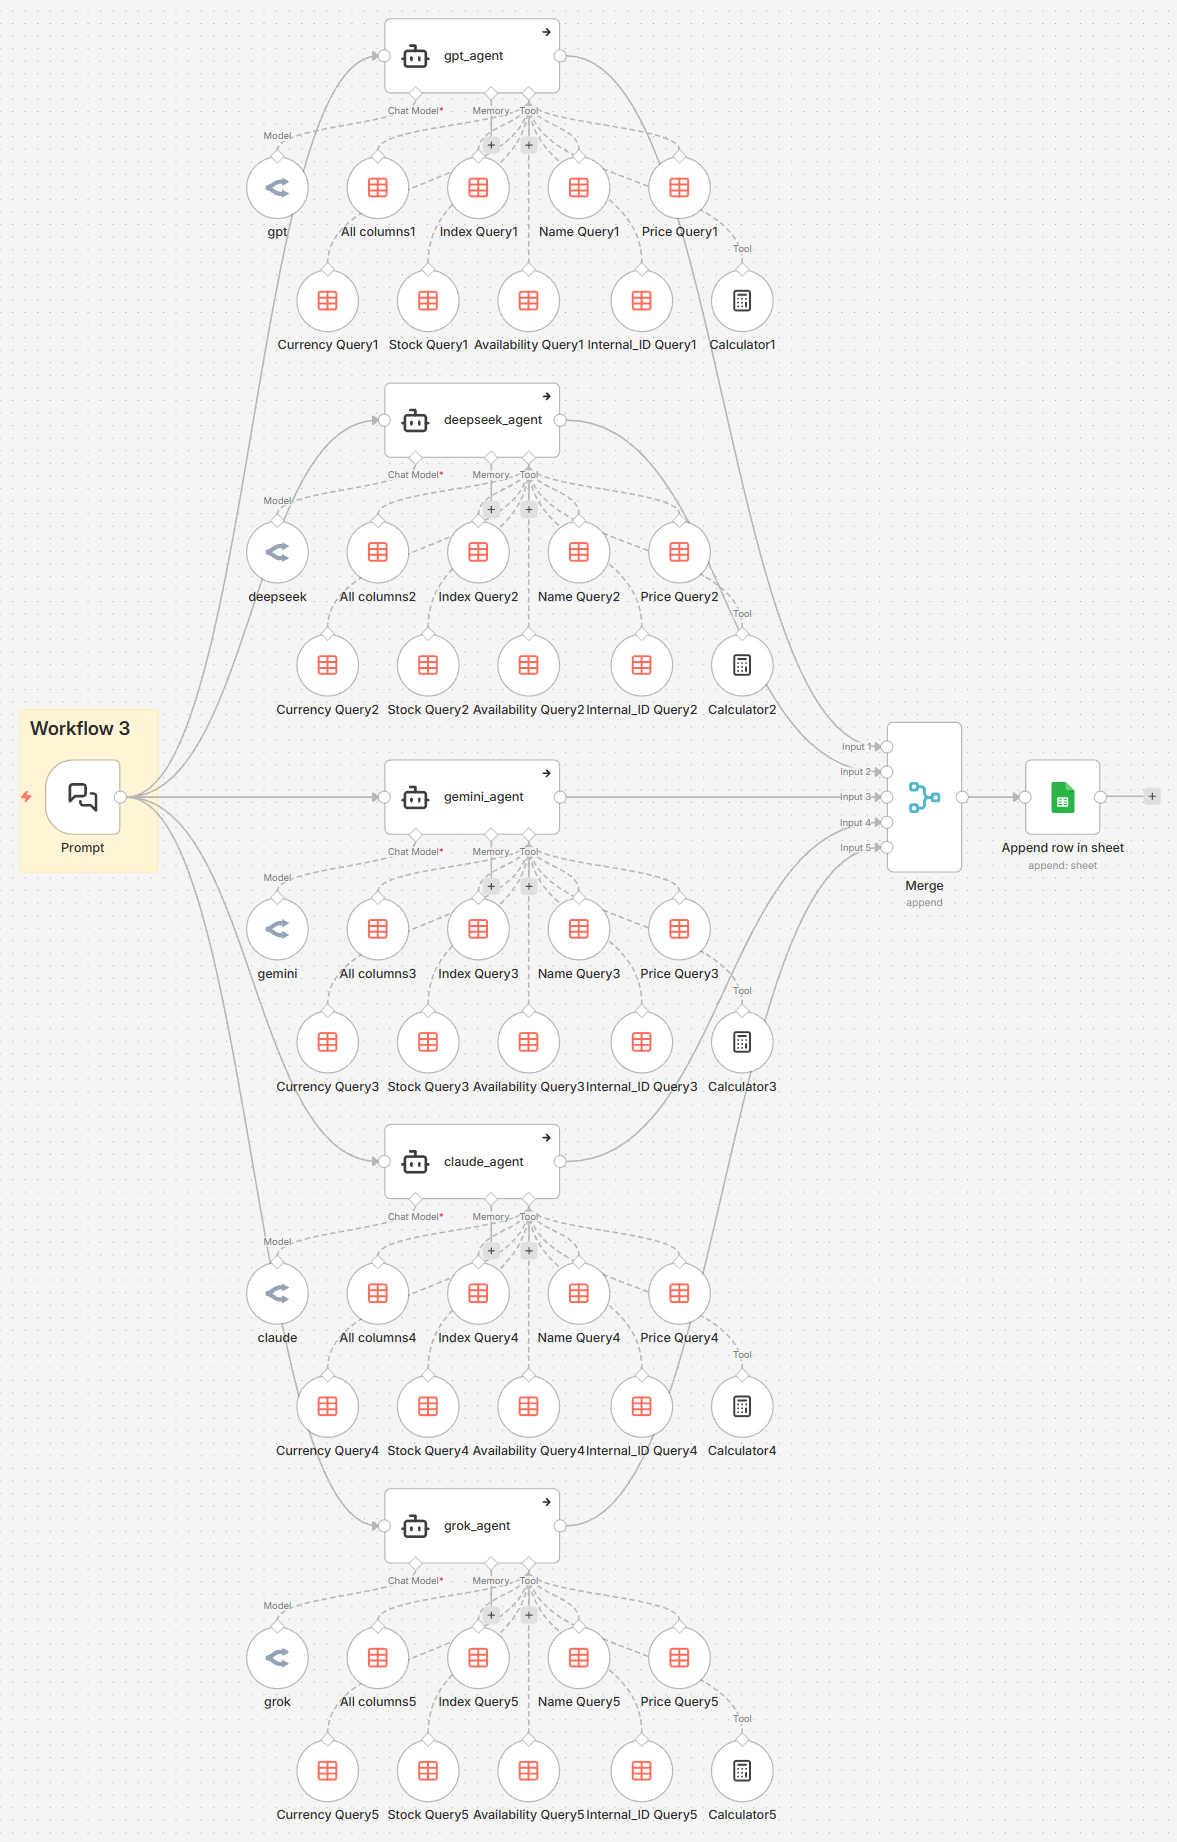
\includegraphics[width=0.6\textwidth]{rysunki/mgr_structured_csv_n8n.png}
        \captionof{figure}{ Scenariusz automatyzacji testów systemów RAG — Workflow 3 dla pliku CSV \cite{n8n}}
        \label{mgr_structured_csv_n8n}
    \end{center}

    W trzecim workflow wydobycie informacji z pliku CSV przechowywanego na tej samej platformie było bardziej skomplikowane. Należało użyć węzłów Data Table Tool, które służyły do wydobycia informacji z konkretnych kolumn pliku. W ramach tego badania, były to tylko kolumny zawierające dane niezbędne do odpowiedzi na zadawane pytania. Podobnie jak w drugim workflow, tutaj także agenty AI korzystały z kalkulatora.

    W ramach powyższych scenariuszy testowych powstało łącznie 30 różnych konfiguracji systemów RAG, po sześć dla każdego badanego modelu LLM. Tabela poniżej \ref{systemy_rag} prezentuje podział i nazwy tych systemów dla wybranych modeli.

    \begin{table}[H]
        \centering
        \caption{ Wykaz 30 implementacji systemów RAG stworzonych dla pięciu wybranych modeli LLM }
        \begin{tabularx}{\textwidth}{|p{4cm}|X|}
        \hline
        \textbf{Model LLM} & \textbf{Dedykowane systemy RAG} \\
        \hline
        gpt-5-mini &  gpt-pdf-openai, gpt-pdf-cohere, gpt-scraped-openai, gpt-scraped-cohere, gpt-sql, gpt-csv \\ \hline
        
        deepseek-v3.2-exp &  deepseek-pdf-openai, deepseek-pdf-cohere, deepseek-scraped-openai, deepseek-scraped-cohere, deepseek-sql, deepseek-csv \\ \hline
        
        gemini-3-flash-preview  &  gemini-pdf-openai, gemini-pdf-cohere, gemini-scraped-openai, gemini-scraped-cohere, gemini-sql, gemini-csv \\ \hline

        claude-haiku-4.5 &  claude-pdf-openai, claude-pdf-cohere, claude-scraped-openai, claude-scraped-cohere, claude-sql, claude-csv \\ \hline

        grok-4.1-fast &  grok-pdf-openai, grok-pdf-cohere, grok-scraped-openai, grok-scraped-cohere, grok-sql, grok-csv \\ \hline
        \end{tabularx}
        \label{systemy_rag}
    \end{table}

    
\cleardoublepage

\chapter{Analiza wyników badania}
W niniejszym rozdziale autor zaprezentował analizę stworzonych systemów RAG pod kątem dokładności, liczby zużytych tokenów, czasu oraz przepustowości podczas generowania odpowiedzi. Warto nadmienić, iż na wykresach kolorem niebieskim oznaczono rezultaty dla systemów RAG zawierających dane nieustrukturyzowane, a czerwonym rezultaty dla systemów RAG zawierających dane ustrukturyzowane.

    
    \section{ Dokładność odpowiedzi }
    W celu zmierzenia dokładności odpowiedzi dużych modeli językowych w systemach RAG, autor pracy oceniał odpowiedzi zero-jedynkowo. Jeżeli odpowiedź była poprawna — trafnie odpowiadała na zadane pytanie — uznawana była za pozytywną (1), a w przeciwnym razie za negatywną (0). Warto podkreślić, że odpowiedzi nie były deterministyczne. Na poniższym rysunku \ref{dokladnosc_wyniki} przedstawiono wykres dokładności w procentach dla konkretnej konfiguracji systemu RAG.

    \begin{center}
        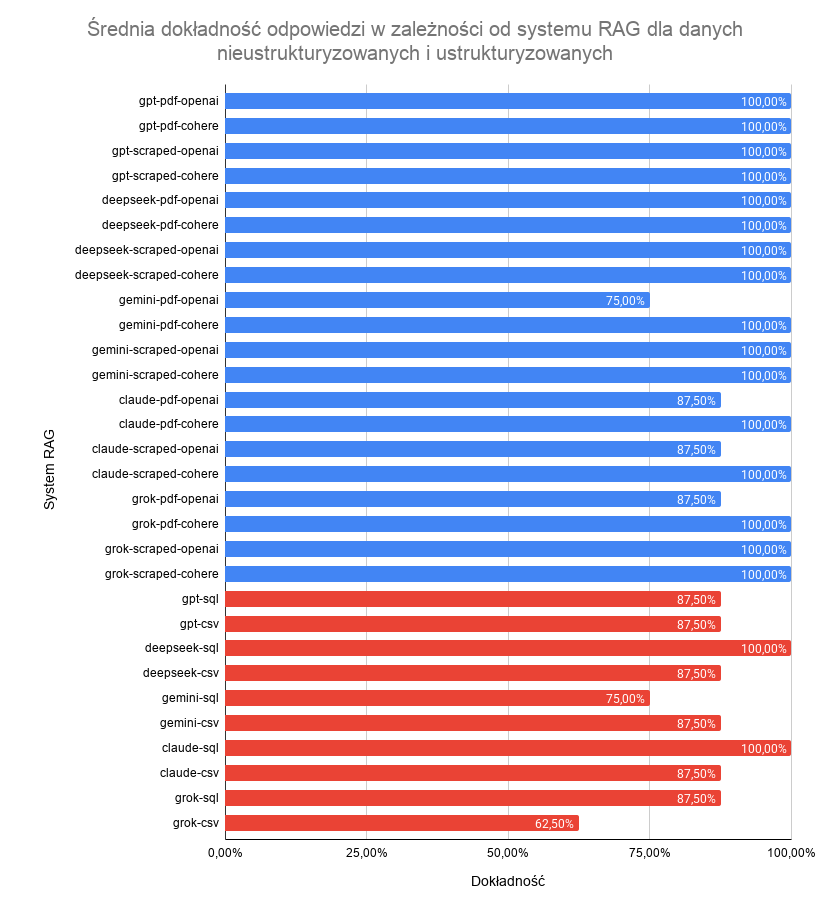
\includegraphics[width=0.8\textwidth]{rysunki/dokladnosc_wyniki.png}
        \captionof{figure}{ Średnia dokładność wygenerowanej odpowiedzi w zależności od systemu RAG dla danych nieustrukturyzowanych i ustrukturyzowanych }
        \label{dokladnosc_wyniki}
    \end{center}

    Zaobserwowano, że badane modele wykazały wysoką zdolność do udzielania poprawnych odpowiedzi na zadane pytania. Aż 18 na 30 konfiguracji RAG poradziło sobie bezbłędnie. Odnosząc się do danych nieustrukturyzowanych, LLMy znacznie lepiej poradziły sobie z interpretacją pliku tekstowego (scraped) niż PDF. Natomiast, w odniesieniu do danych ustrukturyzowanych, odpowiedzi dotyczące pliku SQL były trafniejsze niż te dotyczące pliku CSV. Zdecydowanie lepiej poradziły sobie LLMy przeznaczone do odpowiadania na pytania w oparciu o dane nieustrukturyzowane. Model deepseek-v3.2-exp wyróżnił się największą dokładnością i pomylił się łącznie tylko w jednym pytaniu. W kwestii embeddera, znacznie lepiej poradził sobie model od firmy Cohere niż OpenAI. Systemy RAG wykorzystujące ten embedder wykazały się 100\% skutecznością. Najgorzej wypadła konfiguracja grok-csv, w której model odpowiedział dobrze tylko na pięć z ośmiu pytań (62,50\%). Co ciekawe, drugie pytanie z kategorii integracji informacji okazało się najcięższe dla dużych modeli językowych w ramach nieustrukturyzowanego dokumentu. W czterech odpowiedziach z dwudziestu  padło stwierdzenie, że informacja o liczbie parametrów modelu GPT-1 nie została zawarta w tekście. Z kolei, w ramach pliku CSV, modele nie umiały odpowiedzieć na drugie średniozaawansowane pytanie, gdyż pojawiał się błąd: \enquote{'Price > 920' nie jest liczbą}.


    \section{ Zużycie tokenów }
    W drugim kroku, przeanalizowano koszty — liczbę tokenów zużytych przez modele do interpretacji zapytania i wygenerowania odpowiedzi. Na rysunku \ref{tokeny_wyniki} przedstawiono rezultaty testu.

    \begin{center}
        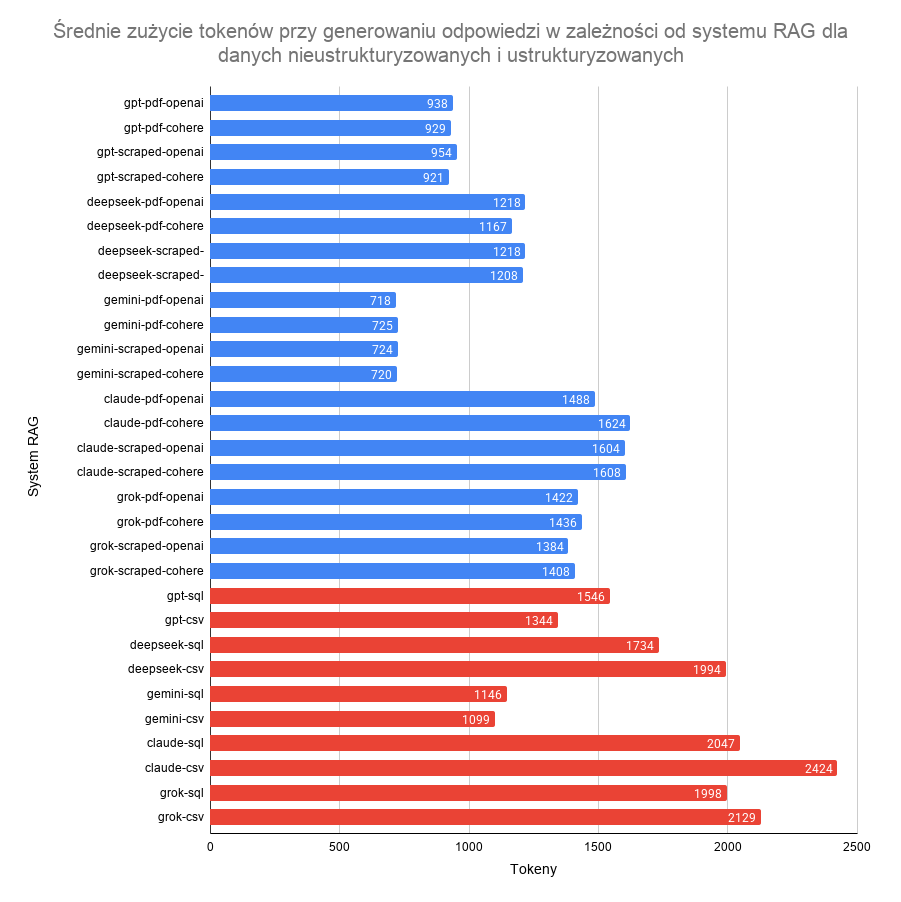
\includegraphics[width=0.88\textwidth]{rysunki/tokeny_wyniki.png}
        \captionof{figure}{ Średnie zużycie tokenów podczas generowania odpowiedzi w zależności od systemu RAG dla danych nieustrukturyzowanych i ustrukturyzowanych }
        \label{tokeny_wyniki}
    \end{center}

    Uzyskane wyniki wskazują, iż znacznie bardziej kosztowne jest stosowanie systemu RAG z danymi ustrukturyzowanymi (średnie zużycie: 1746 tokenów) niż nieustrukturyzowanymi (średnie zużycie: 1171 tokenów). Dla obu rodzajów danych trudno jest jednoznacznie stwierdzić, w ramach których dokumentów wygenerowanie odpowiedzi było najmniej kosztowne. Podobna sytuacja ma miejsce przy określaniu najbardziej wydajnego modelu embeddingowego. Łatwo dostrzec, że systemy stosujące gemini-3-flash-preview wypadają najkorzystniej, ponieważ średnie zużycie wyniosło tylko 855 tokenów. Przeciwieństwo stanowi claude-haiku-4.5, który średnio zużył ponad dwa razy więcej tokenów, aż 1799.
    
    
    \section{ Czas generowania odpowiedzi }
    W kolejnym kroku, porównano systemy RAG pod kątem czasu generowania odpowiedzi. Poniższy rysunek \ref{czas_wyniki} prezentuje te rezultaty.
    
    \begin{center}
        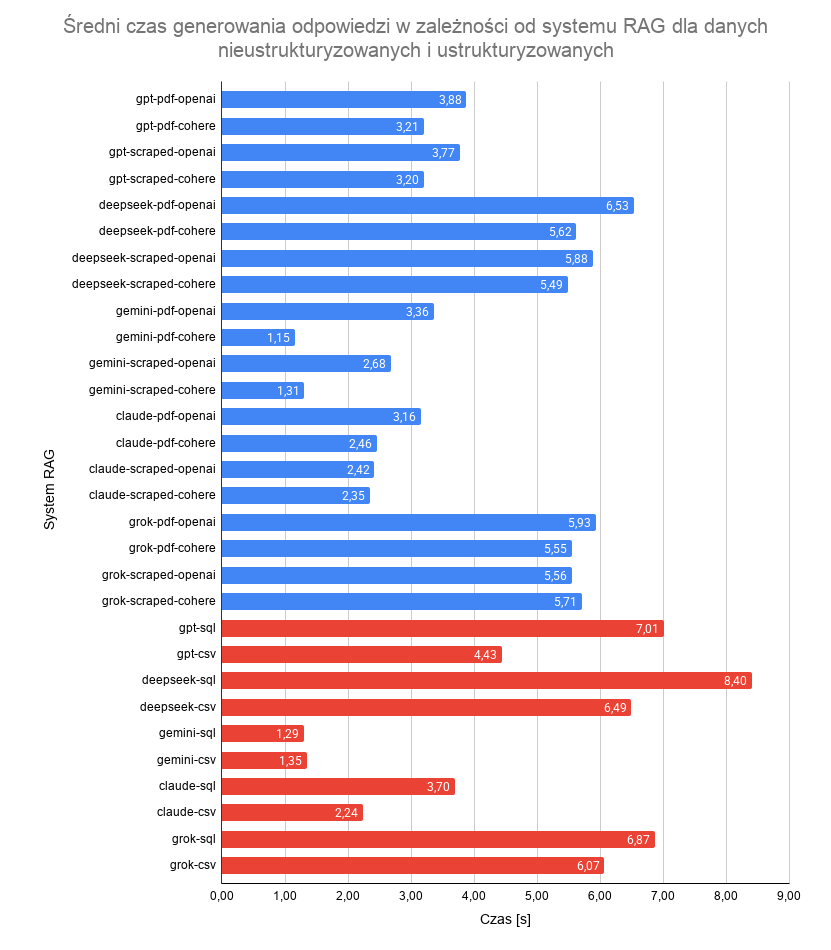
\includegraphics[width=0.8\textwidth]{rysunki/czas_wyniki.png}
        \captionof{figure}{ Średni czas potrzebny na wygenerowanie odpowiedzi w zależności od systemu RAG dla danych nieustrukturyzowanych i ustrukturyzowanych }
        \label{czas_wyniki}
    \end{center}

    Z wykresu wynika, iż znacznie mniej czasochłonne jest wygenerowanie odpowiedzi dla systemów RAG zawierających dane nieustrukturyzowane (średni czas: 3,96 sekund) niż ustrukturyzowane (średni czas: 4,78 sekund). Dla pierwszego rodzaju danych łatwo zauważyć, że odpowiedzi w ramach pliku CSV generowane są znacznie szybciej. Powodem może być fakt hostowania pliku na tej samej platformie, na której było przeprowadzone badanie. Dla drugiego rodzaju danych można zauważyć, że odpowiedzi w ramach pliku tekstowego (scraped) są generowane szybciej. Może to wynikać z jego prostej struktury, charakterystycznej dla plików markdown. Co ciekawe, systemy RAG stosujące embedder od OpenAI są znacznie wolniejsze od analogicznych systemów wykorzystujących embedder od Cohere. Najszybszym modelem okazał się być model gemini-3-flash-preview (średni czas: 1,86 sekund), a najwolniejszym deepseek-v3.2-exp (średni czas: 6,40 sekund).
    
    
    \section{ Przepustowość tokenów }
    W ostatnim kroku, przeanalizowano systemy RAG pod kątem przepustowości tokenów — liczby zużytych tokenów na sekundę — podczas generowania odpowiedzi. Posiadając wyniki z dwóch poprzednich podrozdziałów, można było w łatwy sposób obliczyć przepustowość ze wzoru \ref{wzór_przepustowość_odpowiedzi_llm}. Na poniższym rysunku \ref{przepustowosc_wyniki} zobrazowano wyniki tych obliczeń.
    
    \begin{center}
        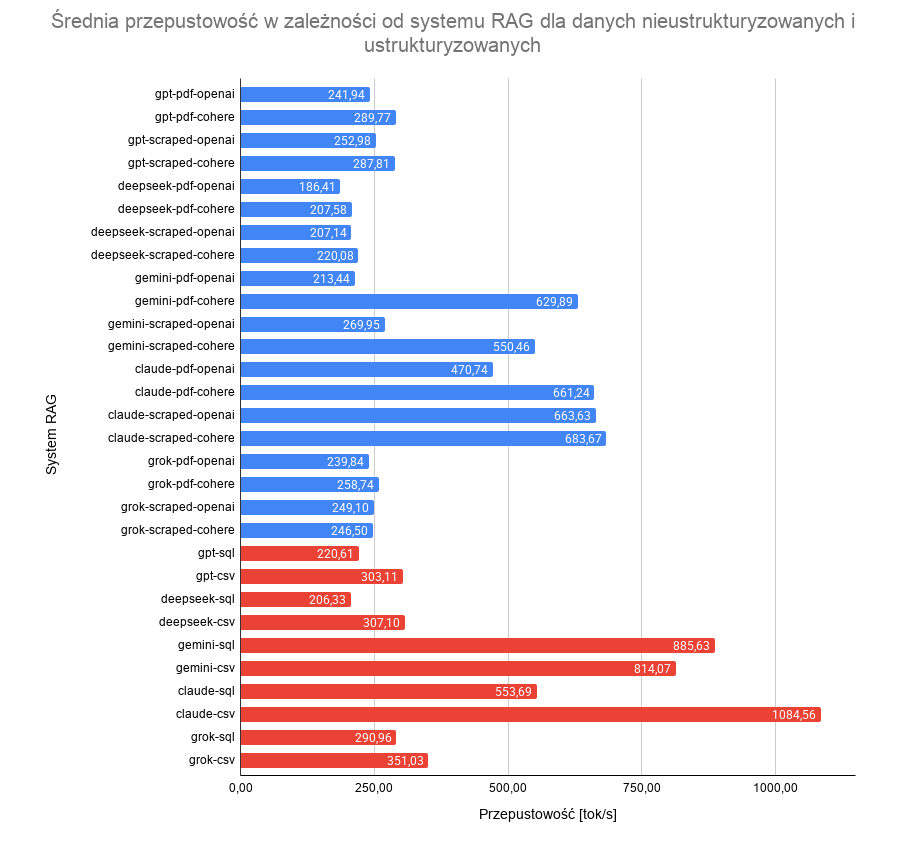
\includegraphics[width=0.9\textwidth]{rysunki/przepustowosc_wyniki.png}
        \captionof{figure}{ Średnia przepustowość w zależności od systemu RAG dla danych nieustrukturyzowanych i ustrukturyzowanych }
        \label{przepustowosc_wyniki}
    \end{center}
    
    Z wykresu wynika, że w przyjętym scenariuszu testowym znacznie większą przepustowością charakteryzują się systemy RAG zawierające dane ustrukturyzowane (średnio 501,71 tok/s) niż te zawierające dane nieustrukturyzowane (średnio 351,54 tok/s). Można zauważyć, że przepustowość była znacznie wyższa dla systemów zawierających plik CSV niż bazę SQL. Dla danych nieustrukturyzowanych dostrzeżono, iż systemy z plikiem tekstowym (scraped) mają niewiele większą przepustowość tokenów (średnio o 23 tok/s) niż te z plikiem PDF. Z wykresu i obliczeń jasno wynika, że embedder od Cohere charakteryzuje się lepszymi wynikami niż embedder od OpenAI w każdej konfiguracji RAG w tym teście. Optymalnym dużym modelem językowym okazał się być claude-haiku-4.5, gdyż średnia przepustowość w związanych z nim systemach wyniosła 686,26 tok/s.
    

    \section{ Wnioski }
    Zaprezentowane przez autora wyniki nie są porównywalne z rezultatami zaprezentowanymi w artykułach \cite{art2_unstructured2024} i \cite{art3_structured2024}. Warto mieć na uwadze, że z racji na ograniczenia czasowe testy wykonywane przez autora pracy dyplomowej zostały przeprowadzone dla każdego rodzaju danych za pomocą tylko ośmiu a nie kilkuset czy nawet kilku tysięcy zróżnicowanych pytań.
    
    Wybrano dwie optymalne konfiguracje RAG spośród badanych. W ramach nieustrukturyzowanych dokumentów za najlepszy system uznano gpt-scraped-cohere. Wyróżnił się stuprocentową dokładnością i generował stosunkowo mało tokenów w krótkim czasie. Natomiast, w ramach danych ustrukturyzowanych za najlepszy system uznano claude-sql. Pomimo zużycia największej liczby tokenów, także zapewnił stuprocentową skuteczność odpowiedzi bardzo szybko odpowiadając na zadane pytania.
        
    
    \section{ Implementacja optymalnego rozwiązania z wykorzystaniem graficznego interfejsu użytkownika }

    Oba systemy RAG, które w poprzednim podrozdziale zostały wybrane za najwydajniejsze spośród badanych konfiguracji, udostępniono za pomocą graficznego interfejsu użytkownika. Stronę wykonano za pomocą narzędzia Lovable \cite{lovable}, a hosting odbywa się lokalnie. Na poniższym rysunku \ref{gui_lovable} przedstawiono GUI wraz z przykładową konwersacją.
    
    \begin{center}
        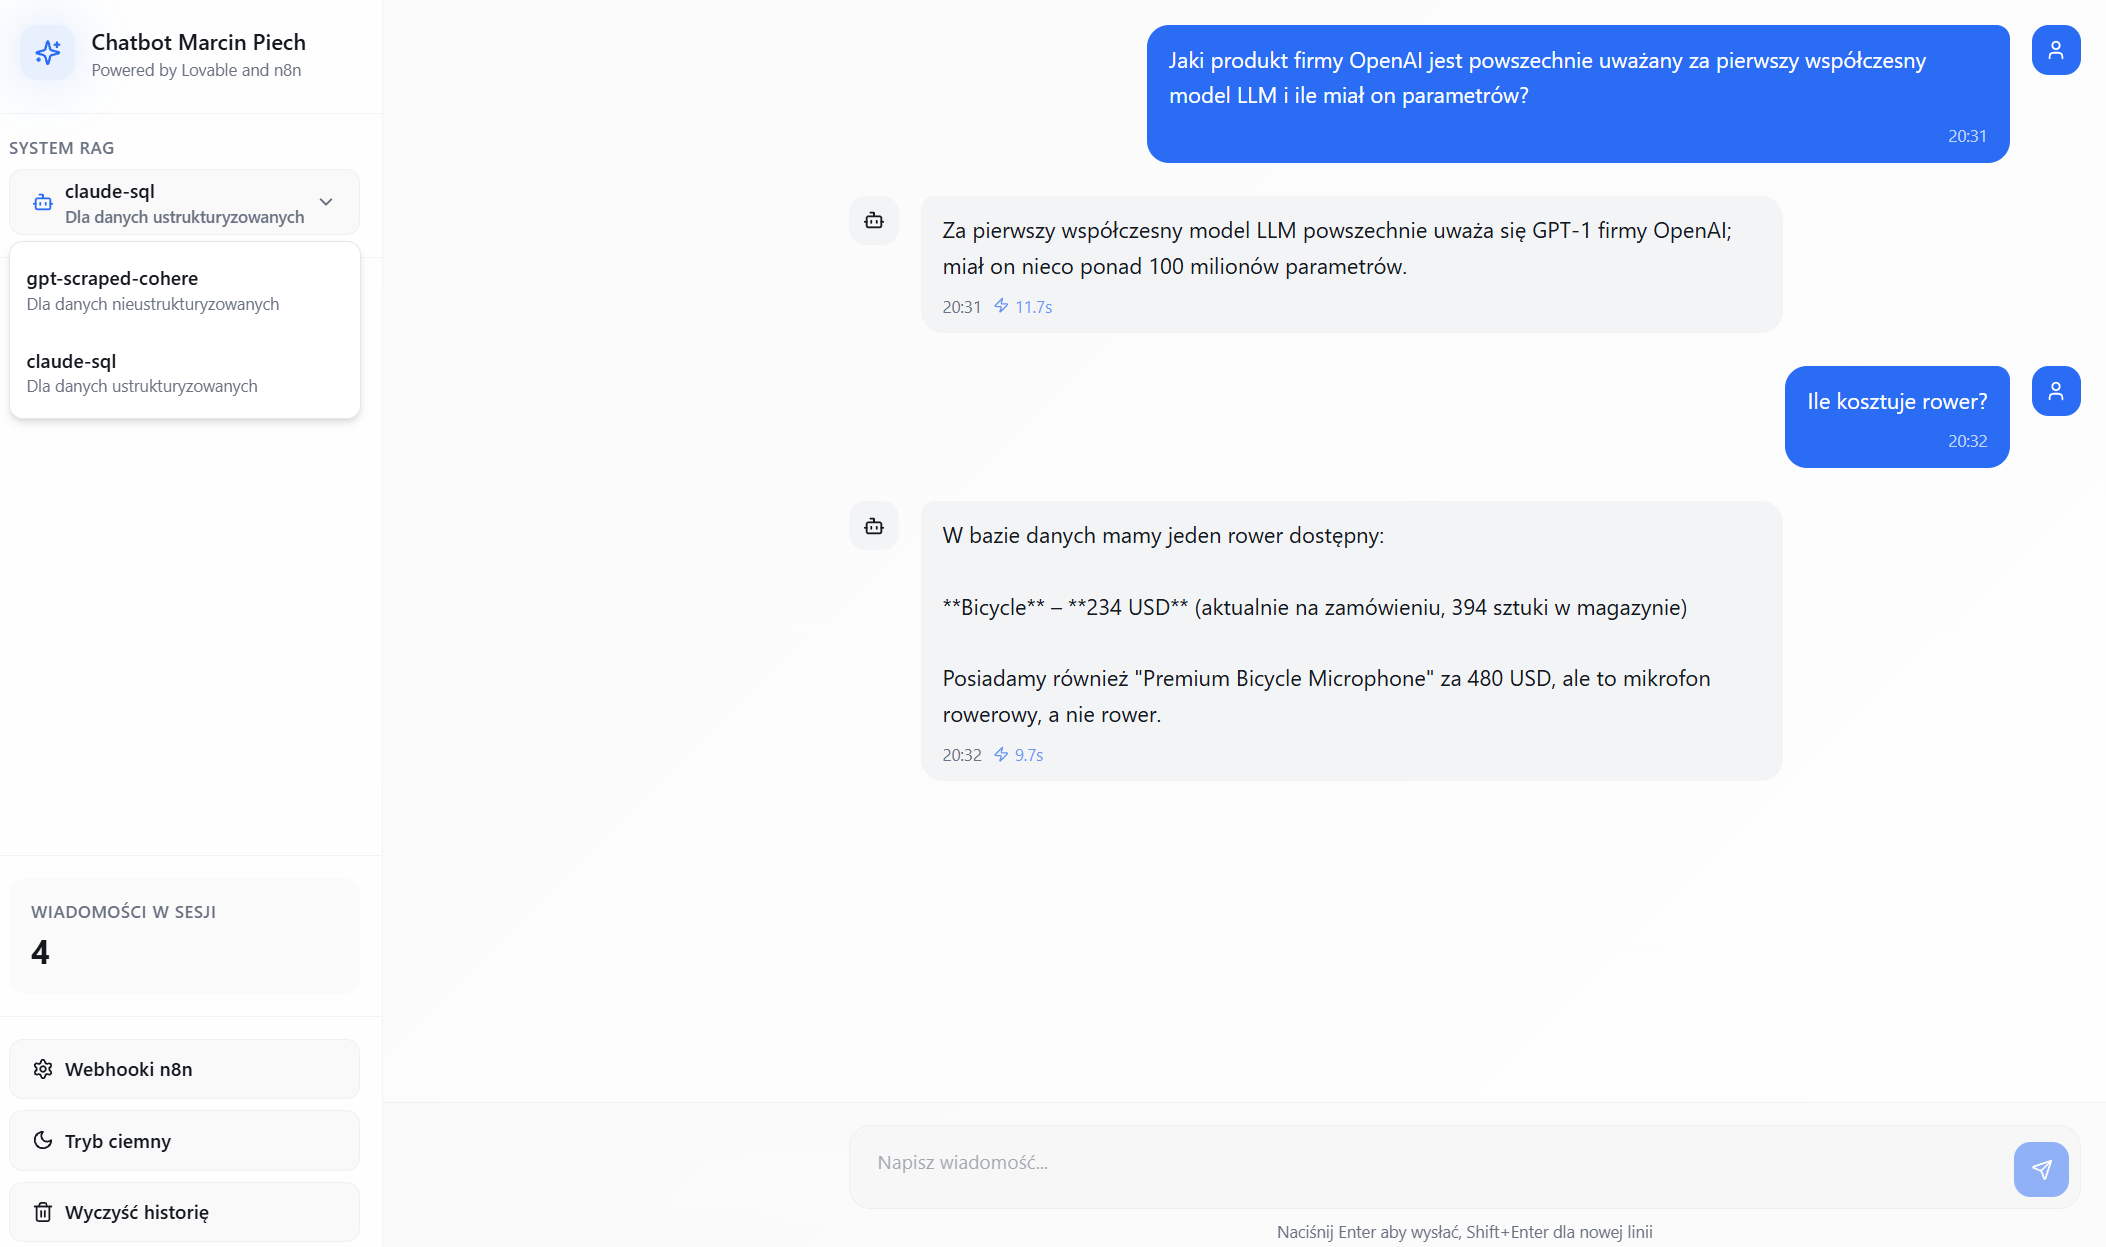
\includegraphics[width=0.9\textwidth]{rysunki/gui_lovable.png}
        \captionof{figure}{ Graficzny interfejs użytkownika służący do implementacji dwóch najwydajniejszych konfiguracji RAG dla danych nieustrukturyzowanych i ustrukturyzowanych \cite{lovable}}
        \label{gui_lovable}
    \end{center}
    
    \noindent Dostępna jest możliwość wyboru systemu RAG, na bazie którego chce się prowadzić konwersację — gpt-scraped-cohere lub claude-sql. Co ciekawe, w ramach jednej konwersacji można prowadzić dialog z dwoma systemami. Na załączonym obrazie \ref{lovable_webhooki_n8n} widnieje tego przykład. Pierwsza wiadomość została wysłana do gpt-scraped-cohere a druga do claude-sql. W lewym dolnym rogu widnieje liczba wiadomości w obecnej sesji, przycisk do zmiany motywu na ciemny oraz przycisk do wyczyszczenia konwersacji (rozpoczęcia dialogu od nowa). Znajdziemy tam także przycisk do konfiguracji adresów URL webhooków z dedykowanego workflow w n8n, które umożliwiają połączenie backendu (program w n8n) z frontendem (interfejs użytkownika).

    \begin{center}
        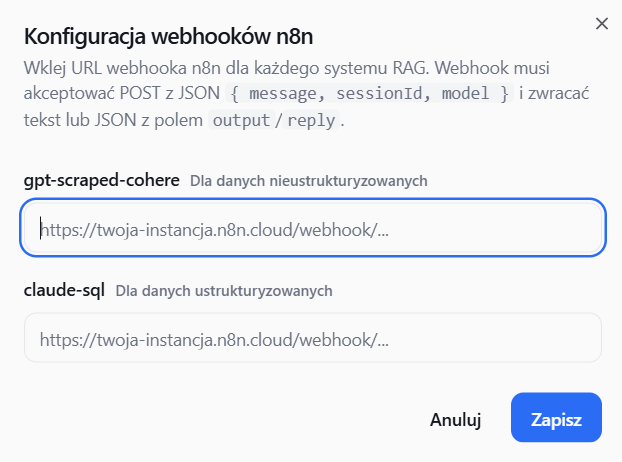
\includegraphics[width=0.45\textwidth]{rysunki/lovable_webhooki_n8n.png}
        \captionof{figure}{ Widok okna służącego do konfiguracji adresów URL webhooków w n8n dedykowanych dla konkretnych systemów RAG \cite{lovable}}
        \label{lovable_webhooki_n8n}
    \end{center}
    
    \noindent Warto zauważyć, że każda z odpowiedzi chatbota zawiera informację o której godzinie została dostarczona i ile czasu zajęło jej wygenerowanie w sekundach. 

    Konwersacja z dwoma dużymi modelami językowymi może się odbywać dzięki wcześniej wspomnianemu oprogramowaniu w n8n. Na poniższym rysunku \ref{mgr_gui_n8n} przedstawiono dwa procesy przetwarzania zapytania. Workflow po lewej stronie, zaczynające się od węzła Webhook1, odzwierciedla wybrany system RAG przeznaczony do danych nieustrukturyzowanych (gpt-scraped-cohere). Workflow po prawej stronie, zaczynający się od węzła Webhook2, reprezentuje wybrany system RAG przeznaczony do danych ustrukturyzowanych (claude-sql).
    
    \begin{center}
        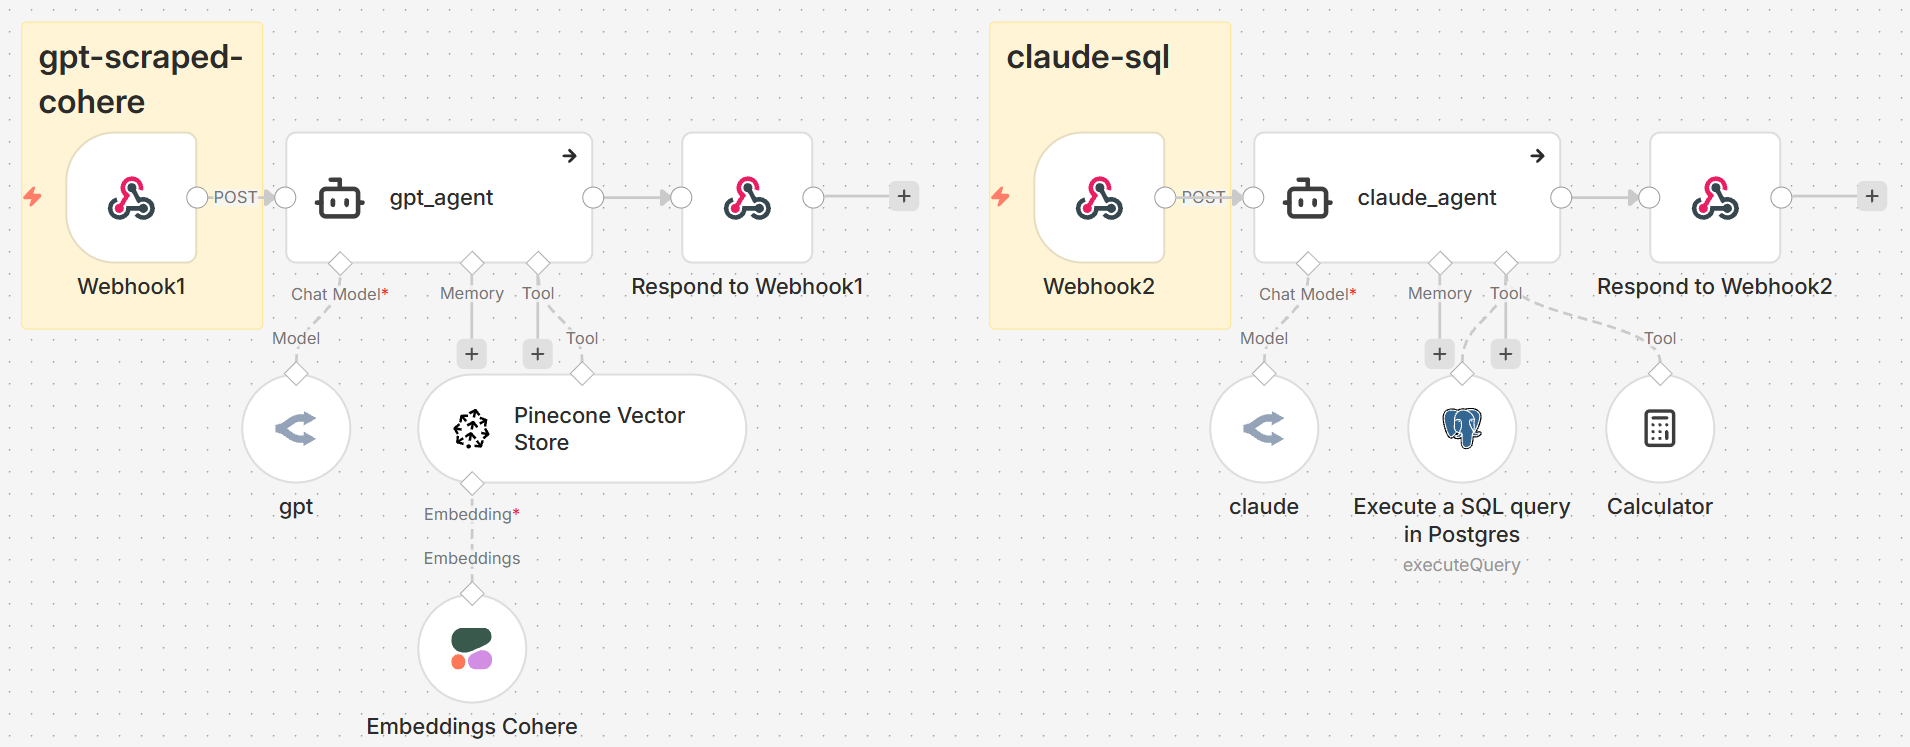
\includegraphics[width=0.9\textwidth]{rysunki/mgr_gui_n8n.png}
        \captionof{figure}{ Oprogramowanie w n8n służące do konwersacji z dwoma najwydajniejszymi konfiguracjami RAG za pomocą graficznego interfejsu użytkownika \cite{n8n}}
        \label{mgr_gui_n8n}
    \end{center}

    Węzły Webhook1 i Webhook2 są ustawione w stan aktywnego nasłuchiwania (published). Warto dodać, iż są one ustawione na odbieranie żądań HTTP metodą POST. Dzięki temu pytanie zadane przez użytkownika poprzez GUI zostaje przekazane w czasie rzeczywistym do konkretnego agenta AI. Następnie, wygenerowana odpowiedź trafia do odpowiedniego węzła Respond to Webhook. Pozwala on przekazać tę wiadomość do GUI, co umożliwia zachowanie ciągłości konwersacji i kolejności wiadomości.
\cleardoublepage

\chapter{Podsumowanie}
Cel niniejszej pracy dyplomowej został spełniony. Dzięki autorskiemu oprogramowaniu do automatyzacji testów, zbadano 30 konfiguracji systemów RAG wykorzystujących pięć najnowszych popularnych modeli językowych firm takich jak: OpenAI, DeepSeek, Google, Anthropic oraz xAI. Ocena wyników opierała się na następujących kryteriach: trafność odpowiedzi, koszt i czas wygenerowania odpowiedzi oraz przepustowość tokenów. Ponadto, poprzez intuicyjny graficzny interfejs użytkownika, zaimplementowano dwa najwydajniejsze systemy RAG: jeden przeznaczony do danych nieustrukturyzowanych oraz drugi do danych ustrukturyzowanych.

Wyniki badania okazały się być zaskakująco dobre, ale nieporównywalne z rezultatami trzech omawianych artykułów naukowych. Uważa się, że istnieje jedna przyczyna takich różnic. Autor w ramach testów odpytał systemy RAG za pomocą łącznie szesnastu autorskich pytań. Natomiast, w publikacjach twórcy użyli ich 360, 1000 czy nawet 4780.

Jeżeli prace w ramach tego tematu byłyby kontynuowane, proponuje się poszerzenie bazy pytań do co najmniej pięciuset, żeby dorównać podejściu stosowanemu w publikacjach. Niesie to za sobą potrzebę zastosowania automatyzacji w następujących obszarach: tworzenie pytań, przekazywanie ich do dedykowanego oprogramowania oraz analiza wyników. Dla pierwszego i trzeciego podejścia niezbędny będzie odrębny LLM i oprogramowanie weryfikujące poprawność odpowiedzi, tak jak to przedstawiono w publikacji \cite{art1_2025} w ramach benchmarku MEBench.



\printbibliography[title={Wykaz literatury}]
\addcontentsline{toc}{chapter}{Wykaz literatury}

\listoffigures
\addcontentsline{toc}{chapter}{Wykaz rysunków}

\listoftables
\addcontentsline{toc}{chapter}{Wykaz tabel}

\end{document}